\documentclass[12pt]{article}
\thispagestyle{empty}

\usepackage{ragged2e}
\usepackage[polish]{babel}
\usepackage{amsfonts}
\usepackage{graphicx}
\usepackage[font=small,labelfont=bf]{caption}
\usepackage{placeins}
\usepackage{xcolor}
\usepackage{multirow}
\usepackage{diagbox}
\usepackage{listings}
\usepackage{hyperref}
\usepackage[a4paper, top=2cm, bottom=2cm]{geometry}
\usepackage{titlesec}
\usepackage{multicol}
\usepackage[T1]{fontenc}

\providecommand{\LastUpdateDate}{NIEZNANA}
\input{LastUpdateDate.tex}

\hypersetup{
    colorlinks,
    citecolor=black,
    filecolor=black,
    linkcolor=black,
    urlcolor=black
}

\begin{document}
\newcommand{\piosenka}[2]{%
  \phantomsection
  \addcontentsline{toc}{subsection}{#1}%
  \subsection*{#2}%
}
\newcommand{\piosenkaSub}[2]{%
  \phantomsection
  \addcontentsline{toc}{subsubsection}{#1}%
  \subsubsection*{#2}%
}

\thispagestyle{empty}
\newgeometry{
  left=0cm,
  right=0cm,
  top=0cm,
  bottom=0cm,
  bindingoffset=0cm,
  twoside=false
}

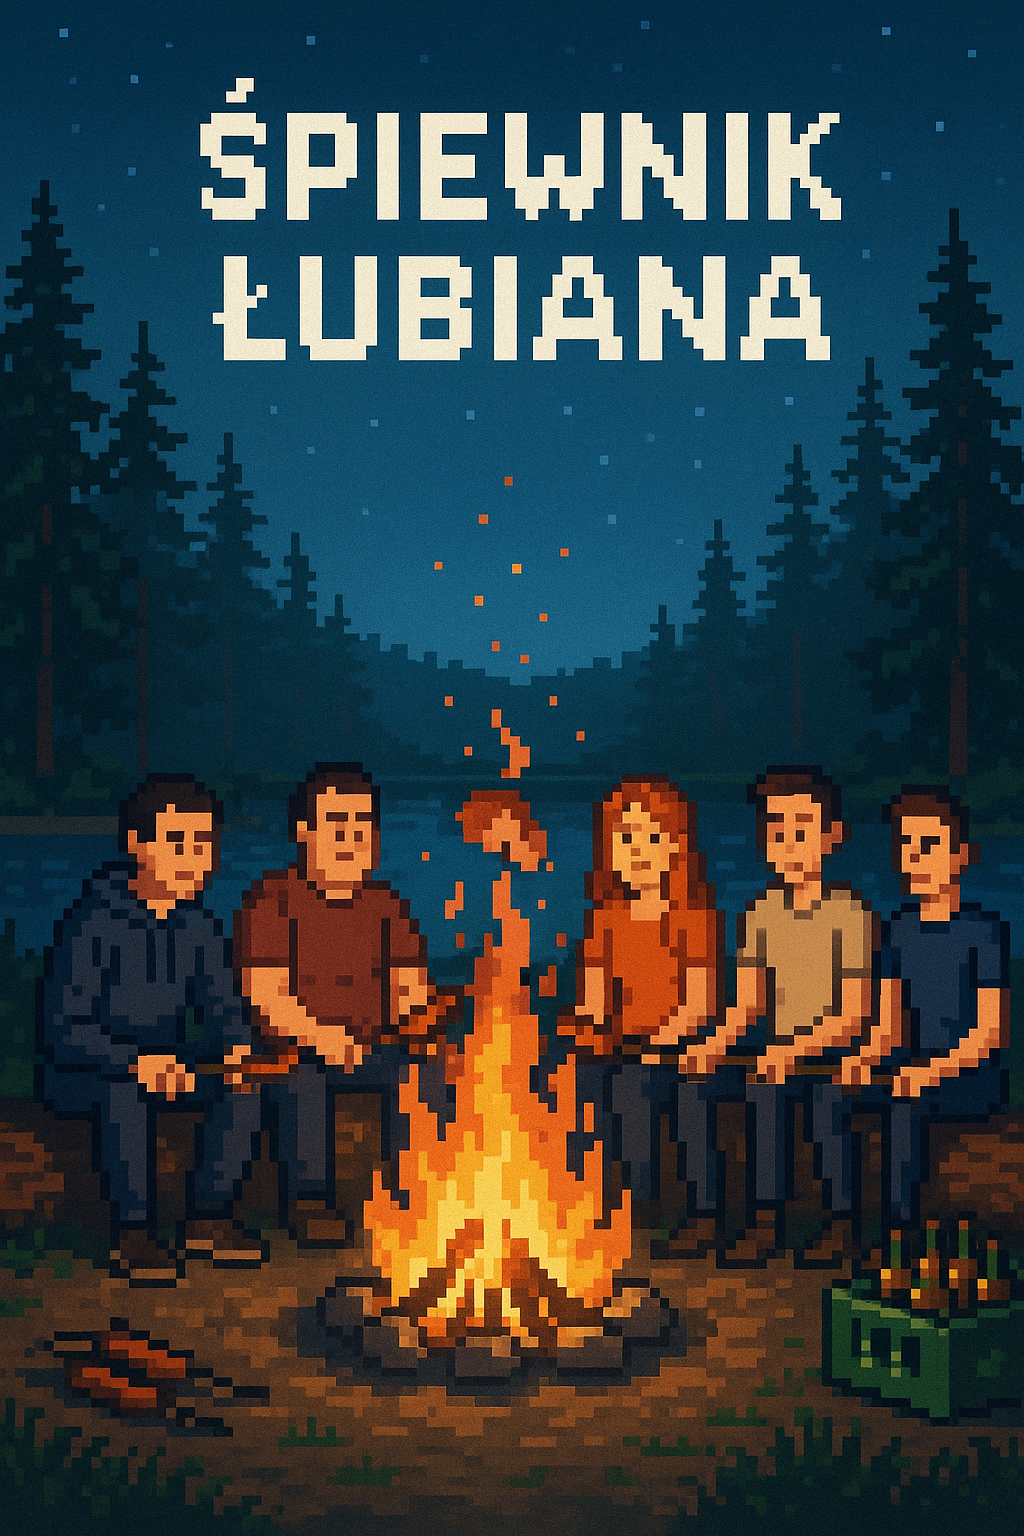
\includegraphics[width=\paperwidth,height=\paperheight]{titlepage.png}

\restoregeometry
\newpage
\thispagestyle{empty}
\ % The empty page

\newpage

\clearpage
\begin{center}

\thispagestyle{empty}
{\fontsize{40}{0} \selectfont Wydanie II}\\
\vspace{0.5cm} 
{\fontsize{20}{0} \selectfont Autorzy: Adam Ziołecki, Damian Panasiuk}
\begin{flushright}
\textit{Wersja z dnia: \LastUpdateDate}
\end{flushright}

\clearpage
\end{center}

\titleformat{\subsection}[block]
  {\centering\fontsize{20}{24}\selectfont\bfseries}
  {}{0pt}{}

\titlespacing*{\subsection}
  {0pt}    %odstęp z lewej (zerowy, bo centrowany)
  {0ex}    %odstęp *nad* (możesz zmienić)
  {6ex}    %odstęp *pod* ← TUTAJ regulujesz przestrzeń pod tytułem

\setlength\parindent{50pt}
\tableofcontents
\clearpage

\phantomsection
\subsection*{Facet to świnia}
\addcontentsline{toc}{subsection}{Big Cyc - Facet to świnia}
\begin{verbatim}
Jak zwykle znów nie robisz nic
Gazetę czytasz cały dzień
Łaskawie czasem obiad zjesz
Po domu snujesz się jak cień
Ty z kolegami wolisz pić
Niż z moją mamą ciasto piec
I zamiast dzieckiem zająć się
Musiałeś znowu wyjść na mecz
To nie jest miłość, lecz ja kocham Cię
Nie jestem świnią, choć ty tego chcesz.

Ref (x2): Facet to świnia
Mówisz, że ty o tym wiesz
Choć ja się staram jak mogę
Przez całe życie słyszę ten tekst

Ty w telewizor gapisz się
A do kościoła chodzisz sam
I nigdy nie przytulisz mnie
W łazience znowu cieknie kran
Gdy w nocy czujesz się jak lew
To obręcz ściska moją skroń
No kiedy wreszcie puścisz mnie
Migrena to najlepsza broń
To nie jest miłość, lecz ja kocham Cię
Nie jestem świnią, choć ty tego chcesz.

Ref (x2): Facet to świnia...

O samochodach mówisz wciąż
Do dziewczyn ślinisz się jak pies
Ty życie zmarnowałeś mi
Od kogo jest ten SMS?
I chociaż oszukujesz mnie
Ja lubię twój szelmowski śmiech
Bez ciebie nudny byłby świat
Bo facet to jest dobra rzecz
To nie jest miłość, lecz ja kocham Cię
Nie jestem świnią, choć ty tego chcesz

Ref (x3): Facet to świnia...
\end{verbatim}
\clearpage

\piosenka{Big Cyc - Dres}{Dres}
\begin{verbatim}
Dresy moje ukochane
Ja zakładam Was nad ranem
Dres mam dres!
Mam trzy paski na ramionach
Każda laska jest już moja
Dres mam dres!
Idę w miasto w moich dresach
zrobię dym w delikatesach
Dres mam dres!
Ten kto nosi Adidasa
To jest facet pierwsza klasa
Dres mam dres!
Moi kumple to kibole
Każdywali się bejsbolem
Dres mam dres!
Punk ucieka hipis zmyka
Kiedy w dresach jest ekipa
Dres mam dres!

Ja noszę dres!
Dres spoko jest!
Ja noszę dres!
Dres modny jest!

W dresach ojciec w dresach matka
W dresach nawet jest sąsiadka
Dres mam dres!
Każdy u nas w dresach chodzi
w dresach starzy w dresach młodzi
Dres mam dres!
I w Szczecinie i na kresach
Cały naród biega w dresach
Dres mam dres!
Wczoraj moja siostra Ola
poszła w dresie do kościoła
Dres mam dres!
Kiedyś w dresach biegał Pele
I Gagarin latał w dresie
Dres mam dres!
Nie wiem drodzy przyjaciele
Co świat mody nam przyniesie
Dres też dres!

Ja noszę dres!
Dres spoko jest!
Ja noszę dres!
Dres modny jest!

Ja noszę dres...
bo wszyscy dresiarze to jedna rodzina
starszy czy młodszy chłopak czy dziewczyna 2x

Ja noszę dres!
Dres spoko jest!
Ja noszę dres!
Dres modny jest! x2
\end{verbatim}
\clearpage

\piosenka{Big Cyc - Makumba}{Makumba}
\begin{verbatim}
Mój ojciec - Makumba - być królem wioski
Ja mieszkać w Afryka, przyjechać do Polski
Żeby studiować w waszym pięknym kraju
Skinheadzi mi tu jednak żyć nie dają
Ja uczyć się ciężko waszego języka
I dostać raz w zęby, gdy iść po ulicach
Polacy rasiści - każdy to powie
I nikt tu nie lubić czarny człowiek

Makumba, Makumba, Makumba ska
Polska - Afryka, Afryka - Polska
Makumba, Makumba, Makumba ska

Ja chcieć uciekać, szykować do drogi
Lecz poznać dziewczyna, co ma piękne nogi
Ja pałać uczuciem i pałać szalenie
I tak się Makumba zakochać w Helenie
My szybko wziąć ślub i mieć dużo dzieci
Rodzice z Afryka przysyłać prezenty
Ja ciągle studiować i uczyć do rana
Hela się
cieszyć z naszego mieszkania

REF. Makumba, Makumba, Makumba ska...

Ja dużo pracować i wiele potrafić
Polska teściowa się o mnie martwić
Ona się ciągle modlić do Boga:
"Boże jedyny, Makumbę zachowaj"

Ja kończyć studia i robić kariera
My mieć samochód i bulteriera
Ja mieszkać tu długo i nie wiedzieć czemu
Nie chcą mnie przyjąć do KPN-u

REF. Makumba, Makumba, Makumba ska...

Polska - Afryka, Afryka - Polska
Makumba, Makumba, ło le, le, le
Makumba, Makumba, ło le, le, le
Makumba, Makumba, ło le, le, le
Makumba, Makumba, ło le, le, le

REF. Makumba, Makumba, Makumba ska...
\end{verbatim}
\clearpage

\piosenka{Big Cyc - Rudy się żeni}{Rudy się żeni}
\begin{verbatim}
Dziś zadzwonił do mnie kumpel i melduje, że Rudy się żeni.
Chociaż ja nie znam kobiety, która chciałaby z nim być.
Rudy klnie, głośno chrapie, ale ona to zmieni.
Bo w kagańcu w potulną owcę, zmienia się dziki lew.

Rudy, Rudy się żeni
Rudy, Rudy się żeni
Rudy, Rudy się żeni
Rudy, Rudy się żeni

Ja nie wierzę w to do dzisiaj, że Rudy się żeni.
On pił piwo, słuchał punka i lubił się bić.
Ale ona go kocha i ona to zmieni.
Bo w tresera rękach nawet dziki tygrys jest smutny jak pies.

Rudy, Rudy się żeni...

Straciliśmy przyjaciela, bo Rudy się żeni.
Już nie będzie wspólnych balang i wypadów na mecz.
Przecież Rudy ją kocha, ale ona to zmieni.
Tylko kumple z nim zostaną, na dobre i złe.

Rudy, Rudy się żeni...
\end{verbatim}
\clearpage

\piosenka{Brathanki - W kinie, w Lublinie}{W kinie, w Lublinie}
\begin{verbatim}
O świcie i o zmroku
O świcie i o zmroku
W południe, w nocy, o świcie
W Skarżysku i w Sanoku
W Skarżysku i w Sanoku
Ty mnie pokochaj nad życie

W berecie, w czapce, chustce
W berecie, w czapce, chustce
W czapce od stryjka ze Lwowa
Na falochronie w Ustce
Na falochronie w Ustce
Ty mnie pokochaj od nowa

W kinie, w Lublinie – kochaj mnie
W Kłaju, w tramwaju – kochaj mnie
Nie marudź, nie szlochaj,
ale z całej siły kochaj
W gminie, w Kętrzynie – kochaj mnie
W metrze i w swetrze – kochaj mnie
Czy miasto czy wiocha, ty mnie z całej siły kochaj

W radości no i w smutku
W radości no i w smutku
W radości z ciepłego lata
Na piasku plaży, w Gródku
Na piasku plaży, w Gródku
Kochaj mnie do końca świata

W spokoju oraz w niebie
W spokoju oraz w niebie
W spokoju palmowych niedziel
W Marwałdzie i w Giętlewie
W Marwałdzie i w Giętlewie
Kochaj w bogactwie i w biedzie

W kinie, w Lublinie – kochaj mnie
W Kłaju, w tramwaju – kochaj mnie
Nie marudź, nie szlochaj,
ale z całej siły kochaj
W gminie, w Kętrzynie – kochaj mnie
W metrze i w swetrze – kochaj mnie
Czy miasto czy wiocha, ty mnie z całej siły kochaj

Jak młody ułan dzielnie
Jak młody ułan dzielnie
Jak wartki na wiosnę strumień
Na nartach wodnych w Mielnie
Na nartach wodnych w Mielnie
Kochaj najmocniej, jak umiesz

Latem w przydrożnym rowie
Latem w przydrożnym rowie
Zimą na sankach i nartach
Najmocniej zaś w Krakowie
Najmocniej zaś w Krakowie
Kochaj, bom tego jest warta

W kinie, w Lublinie – kochaj mnie
W Kłaju, w tramwaju – kochaj mnie
Nie marudź, nie szlochaj,
ale z całej siły kochaj
W gminie, w Kętrzynie – kochaj mnie
W metrze i w swetrze – kochaj mnie
Czy miasto czy wiocha, ty mnie z całej siły kochaj!
\end{verbatim}
\clearpage

\piosenka{Brathanki - Czerwone korale}{Czerwone korale}
\begin{verbatim}
Czerwone korale, czerwone niczym wino
Korale z polnej jarzębiny
I łzy dziewczyny i wielkie łzy

Z miasta płaszcz i korale me
On pochwalił i rzekł
Że ze mną zatańczyć chce
Jego dżins i mej bluzki biel
Zwarły się w tangu wnet
We włosy miał wtarty żel

Potem mnie na wycieczkę wziął
I na wycieczce tej
Mą bieluśką bluzkę zmiął
Wszyscy mi zazdrościli tam
Gdy wróciłam i gdy
W pomiętej bluzeczce szłam

Czerwone korale, czerwone niczym wino
Korale z polnej jarzębiny
I łzy dziewczyny i wielkie łzy

Wczoraj też na tych tańcach był
A na włosach mu żel
Jak srebrzysty księżyc lśnił
Tyle, że z Kryśką cały czas
Tańczył, a w stronę mą
Nie spojrzał ni jeden raz

Z innym zatańczę gdy
Z tą Kryśką będziesz ty
A potem czemu nie
Niech inny mą bluzkę zmnie

Laj laj laj laj la laj
Naj naj naj naj na naj
Na na na naj na naj
Na na na na na na na naj naj naj
\end{verbatim}
\clearpage

\piosenka{Budka suflera - Bal wszystkich świętych}{Bal wszystkich świętych}
\begin{verbatim}
Ta niedziela jest jak film, tani klasy "B",
Facet się pałęta w nim w nieciekawym tle,
Scenarzysta forsę wziął, potem zaczął pić
I z dialogów wyszło dno, zero, czyli nic.

Wszyscy święci balują w niebie,
Złoty sypie się kurz,
A ja włóczę się znów bez Ciebie
I do piekła mam tuż.

Tak bym chciał Cię spotkać raz, w ten jedyny dzień
Lub o tydzień cofnąć czas, ale nie da się,
Chociaż samotności smak aż do bólu znam,
Kiedy innych niedziel brak, trudno, co mi tam...

Wszyscy święci balują w niebie,
Złoty sypie się kurz,
A ja włóczę się znów bez Ciebie
I do piekła mam tuż.

Świat się tylko już ze mną kręci,
Gwiazdy płoną jak stal,
Skasowałaś mnie w swej pamięci,
Aż mi siebie jest żal.

W niebie dzisiaj wszyscy, wszyscy świeci mają bal
W niebie dzisiaj wszyscy, wszyscy świeci mają bal

Wszyscy święci balują w niebie,
Złoty sypie się kurz,
A ja włóczę się znów bez Ciebie
I do piekła mam tuż.

Świat się tylko już ze mną kręci,
Gwiazdy płoną jak stal,
Skasowałaś mnie w swej pamięci,
Aż mi siebie jest żal.

W niebie dzisiaj wszyscy, wszyscy świeci mają bal.
W niebie dzisiaj wszyscy, wszyscy świeci mają bal.
W niebie dzisiaj wszyscy, wszyscy świeci mają bal.
W niebie dzisiaj wszyscy, wszyscy świeci mają bal.
\end{verbatim}
\clearpage

\piosenka{Budka suflera - Jolka, Jolka}{Jolka, Jolka}
\begin{verbatim}
Jolka, Jolka, pamiętasz lato ze snu,
Gdy pisałaś: "tak mi źle,
Urwij się choćby zaraz, coś ze mną zrób,
Nie zostawiaj tu samej, o nie".

Żebrząc wciąż o benzynę, gnałem przez noc,
Silnik rzęził ostatkiem sił,
Aby być znowu w Tobie, śmiać się i kląć,
Wszystko było tak proste w te dni.

Dziecko spało za ścianą, czujne jak ptak,
Niechaj Bóg wyprostuje mu sny!
Powiedziałaś, że nigdy, że nigdy aż tak
słodkie były, jak krew Twoje łzy

Emigrowałem z objęć Twych nad ranem,
Dzień mnie wyganiał, nocą znów wracałem,
Dane nam było, słońca zaćmienie,
Następne będzie, może za sto lat.

Plażą szły zakonnice, a słońce w dół,
Wciąż spadało nie mogąc spaść,
Mąż tam w świecie za funtem, odkładał funt,
Na Toyotę przepiękną, aż strach.

Mąż Twój wielbił porządek i pełne szkło,
Narzeczoną miał kiedyś, jak sen,
Z autobusem Arabów* zdradziła go,
Nigdy nie był już sobą, o nie

Emigrowałem z ramion Twych nad ranem,
Dzień mnie wyganiał, nocą znów wracałem,
Dane nam było, słońca zaćmienie,
Następne będzie, może za sto lat.

W wielkiej żyliśmy wannie i rzadko tak,
Wypełzaliśmy na suchy ląd,
Czarodziejka gorzałka tańczyła w nas,
Meta była o dwa kroki stąd.

Nie wiem ciągle dlaczego zaczęło się tak,
Czemu zgasło też nie wie nikt,
Są wciąż różne koło mnie, nie budzę się sam,
Ale nic nie jest proste w te dni.
\end{verbatim}
\clearpage

\piosenka{Budka suflera - Takie tango}{Takie tango}
\begin{verbatim}
Na sali wielkiej i błyszczącej
Tak jak nocne Buenos Aires
Które nie chce spać
Orkiestra stroi instrumenty
Daje znak i zaraz zacznie
Nowe tango grać

Siedzimy obok obojętni
Wobec siebie jak turyści
Wystukując rytm
Nie będzie tanga między nami
Choćby nawet cud się ziścił
Nie pomoże nic

Chociaż płyną ostre nuty
W żyłach płonie krew
Nigdy żadne z nas do tańca
Nie poderwie się

Ref.
Bo do tanga trzeba dwojga
Zgodnych ciał i chętnych serc
Bo do tanga trzeba dwojga
Tak ten świat złożony jest

Zaleje w końcu Buenos Aires
Noc tak gęsta jak atrament
A gdy przyjdzie brzask
Co było w naszych sercach kiedyś,
Kiedyś jak świecący diament
Cały straci blask

I choć będą znowu grali
Bóg to jeden wie
Nigdy razem na tej sali
Nie spotkamy się

Ref.
Bo do tanga trzeba dwojga
Zgodnych ciał i chętnych serc
Bo do tanga trzeba dwojga
Tak ten świat złożony jest /x4
\end{verbatim}
\clearpage

\piosenka{Ivan i Delfin - Jej czarne oczy}{Jej czarne oczy}
\begin{verbatim}
Złe kilometry dzielą nas
Lato umiera jesieni czas
W blaszany daszek tłucze deszcz
A w mojej głowie wciąż ktoś jest
Więc gdy wspomnienia męczą cię
Wracają myśli krótkie dnie
Zobaczyć jeszcze raz

Jej piękne czarne oczy
Śnią się czarne oczy
Ich nie przeoczysz
Wiem że nie
Jej piękne czarne oczy
Widzę czarne oczy
To za mną kroczy
Ze mną jest (2x)

Takie to życie dziwne jest
Miłość tęsknota ścigają się
Możesz uciekać możesz nie
Jedno i drugie dopadnie cię
Wiec gdy wspomnienia męczą cię
Wracają myśli krótkie dnie
Zobaczyć jeszcze raz

Jej piękne czarne oczy
Śnią się czarne oczy
Ich nie przeoczysz
Wiem że nie
Jej piękne czarne oczy
Widzę czarne oczy
To za mną kroczy
Ze mną jest (2x)

Więc gdy wspomnienia
Męczą cię
Wracają myśli, krótkie dnie
Zobaczyć jeszcze raz
Jej piękne, czarne, oczy...

Jej piękne czarne oczy... (2x)
\end{verbatim}
\clearpage

\piosenka{Zenek Martyniuk - Miłość w Zakopanem}{Miłość w Zakopanem}
\begin{verbatim}
Teraz już wszystko wiem
Bawiłem grubo się i w Ameryce, (USA)
Gdzieś pod palmami raj
Mówili jedź, bo tam podobno życie (ooo)

To był przepiękny czas
Życie tętniło w nas
Pamiętasz miła
Lecz to w ojczyźnie właśnie nam się przydarzyła

Miłość, Miłość w Zakopanem
Polewamy się szampanem
Rycerzem jestem ja
A ty królową nocy
Miłość żarzy w twoje oczy
Rozpędzona jak motocykl
Hej wypijemy wszyćkie drinki aż do dna

Cekiny błyszczą twe
Uśmiechem kusisz mnie
Didżej przygrywa (didżej przygrywa)

Splecione ciała dwa
Tak piękni: ty i ja
szczęście nadpływa

choć na parkiecie tłum
tu dzisiaj oprócz nas nikogo nie ma
cześć tu Sławomir
a w mych ramionach Magdalena

Miłość, Miłość w Zakopanem...

Poranek, jasny świt,
Głowy leciutkie, bo
To przecież góry
Na niebie słońce lśni
Ty jesteś dzisiaj nim
Przeganiasz chmury
Buzi mi teraz daj
A potem więcej, gdy będziemy sami
Bo od wieczora, bejbe, znowu zaczynamy

Miłość, Miłość w Zakopanem... (2x)
\end{verbatim}
\clearpage


\piosenka{Mig - Miód malina}{Miód malina}
\begin{verbatim}
1. Uderzam na imprezę, bo tam nie będę sam.
Zawieszam nagle oko, na widok jednej z dam.
Takiej seksownej lali, nie było dawno tu.
Jej widok mnie zniewolił, aż mi zabrakło tchu.

Ref. Co to jest za dziewczyna, czy ktoś podpowie mi?
Gdy ciało swe wygina - miód malina!
I nie ma drugiej takiej, co ciało takie ma.
Nie mogę się powstrzymać - miód malina! / x2

2. Ona jest przy mnie blisko, na balet przyszedł czas.
Tańczymy w rytmie disco, super imprezka, lans.
Przy takiej ładnej niuni zaczynam w końcu żyć.
Wiem jedno doskonale, tej nocy chcę z nią być.

Ref. Co to jest za dziewczyna, czy ktoś podpowie mi?
Gdy ciało swe wygina - miód malina!
I nie ma drugiej takiej, co ciało takie ma.
Nie mogę się powstrzymać - miód malina! / x2

Co to jest za dziewczyna? czyna czyna
Co to jest za dziewczyna? czyna czyna
Miód malina!

Co to jest za dziewczyna, czy ktoś podpowie mi?
Gdy ciało swe wygina - miód malina!
I nie ma drugiej takiej, co ciało takie ma.
Nie mogę się powstrzymać - miód malina! / x2
\end{verbatim}
\clearpage

\piosenka{Akcent - Przez Twe oczy zielone}{Przez Twe oczy zielone}
\begin{verbatim}
Odkąd zobaczyłem ciebie
Nie mogę jeść, nie mogę spać
Jak do tego doszło, nie wiem?
Miłość o sobie dała znać

Co poradzić mogę na to
Że miłość przyszła właśnie dziś
Że w sercu mym jest lato
A w moich myślach jesteś ty

Przez twe oczy, te oczy zielone oszalałem
Gwiazdy chyba twym oczom oddały cały blask
A ja serce miłości spragnione ci oddałem
Tak zakochać, zakochać się można tylko raz

W mych ramionach cię ukryję
U stóp Ci złożę cały świat
Serce me dla ciebie bije
I czeka na twój mały znak.

Jeden uśmiech twój wystarczy
I moje serce gubi rytm
O twą miłość będę walczył
O miłość walczyć to nie wstyd

Przez twe oczy, te oczy zielone oszalałem
Gwiazdy chyba twym oczom oddały cały blask
A ja serce miłości spragnione ci oddałem
Tak zakochać, zakochać się można tylko raz
(2x)
\end{verbatim}
\clearpage

\piosenka{Disney - Jestem kimś (Planeta Skarbów)}{Jestem kimś (Planeta Skarbów)}
\begin{verbatim}
Świat jest zagadką tak jak ja
Każda chwila jest jak skarb
A marzenia to wszystko, co mam
A mów sobie zdrów przez cały czas
Ja nie słucham cię i tak
I nie będę tym kim chciałbyś ty, żebym był
Uwierz mi

I nie jestem chłopcem, mówię wam
Lecz mężczyzną, honor mam
Więc nie można tak pomiatać mną
No jak mam się uczyć, jeśli nikt
Nie pokaże mi tu nic?
Więc w marzenia uciekam stąd

Bo ja chcę nareszcie zacząć żyć
Pełną piersią, z całych sił
Chcę być wolny i znać szczęścia smak
Co dzień każda chwila zmienia mnie
A świat za mną w tyle jest
Jestem sobą
I jestem kimś

Ja wciąż mogę zdobyć to, co chcę
Czego ty nie możesz mieć
Teraz znasz mnie, lecz nie boję się
Co ty możesz wiedzieć o mnie? Nic
Czy potrafisz pomóc mi?
Jestem sobą tak długo jak wiem kim chcę być

No przestańcie wreszcie truć
Dosyć już pustych słów
Ludzie mówią i kłamią
A życie podobno to sen
A ja wierzę w marzenia
Że to, czego pragnę ma sens

Bo ja chcę nareszcie zacząć żyć
Pełną piersią, z całych sił
Chcę być wolny i znać szczęścia smak
I nie mówcie, że nie zmieniam się
Taki sam wasz każdy dzień
Jestem sobą i jestem kimś
Jestem tu i jestem kimś
Jestem kimś
Jestem kimś
\end{verbatim}
\clearpage

\piosenka{Disney - Zrobię mężczyzn z was (Mulan)}{Zrobię mężczyzn z was (Mulan)}
\begin{verbatim}
To jeszcze daleka droga przed nami
1.
Brać się do roboty,
Wroga bić już czas.
Widzę zamiast mężczyzn mnóstwo bab wśród was.
Takiej bandy nikt nie zlęknie się,
Zadrżyjcie więc na dźwięk tych słów:
MĘŻCZYZN Z WAS WKRÓTCE SAM ZROBIĘ ZNÓW!

2.
Z wierzchu masz być skałą,
Ma się żar w niej tlić.
Każdy bój zwyciężysz,
Zawsze tak ma być.
Dziś, gdy widzę was nie dobrze mi,
Lecz wytężcie wreszcie słuch:
MĘŻCZYZN Z WAS WKRÓTCE SAM ZROBIĘ ZNÓW!

3.
- Co chwila to zatyka mnie.
- Ja ostatnio czuję dreszcze.
- Nie raz z w-fu wiałem, byłem głąb.
- Ten gość dał im nieźle w kość.
- Może mnie nie przejrzał jeszcze.
- Nie chodziłem na pływalnię, to był błąd!

Ref. :
(Silny bądź!)
Musicie być jak szalona rzeka.
(Silny bądź!)
Jak tajfun, który obali mur!
(Silny bądź!)
A równocześnie tak tajemniczy
Jak księżyc, co wygląda tu zza chmur!

4.
Blisko już do walki,
Naprzód gna ten czas.
Tylko twardy rozkaz,
Łączy mnie i was.
Lepiej odejdź, bo
Dla ciebie brak
Miejsca, więc gnaj stąd co tchu.
Z ciebie nic nie da się, zrobić tu!

Ref. : (Silny bądź!)... x2
\end{verbatim}
\clearpage

\piosenka{Dżem - Wehikuł czasu}{Wehikuł czasu}
\begin{verbatim}
Pamiętam dobrze ideał swój.
Marzeniami żyłem jak król.
Siódma rano - to dla mnie noc,
Pracować nie chciałem, włóczyłem się.

Za to do puszki zamykano mnie.
Za to zwykle zamykano mnie.
Po knajpach grywałem za piwko i chleb,
Na szyciu bluesa tak mijał mi dzień.

Ref.
Tylko nocą do klubu "Puls"
Jam-session do rana, tam królował blues
To już minęło, ten klimat, ten luz.
Wspaniali ludzie nie powrócą,
Nie powrócą już!

Lecz we mnie zostało coś z tamtych lat,
Mój mały, intymny, muzyczny świat.
Gdy tak wspominam ten miniony czas,
Wiem jedno, że to nie poszło w las.

Dużo bym dał, by przeżyć to znów -
Wehikuł czasu - to byłby cud!
Mam jeszcze wiarę, odmieni się los,
Znów kwiatek do lufy wetknie im ktoś

Ref.
Tylko nocą do klubu "Puls"
Jam-session do rana, tam królował blues
To już minęło, te czasy, ten luz.
Wspaniali ludzie nie powrócą,
Nie powrócą już! Nie!

Ref.
Tylko nocą do klubu "Puls"
Jam-session do rana, tam królował blues
To już minęło, te czasy, ten luz.
Wspaniali ludzie nie powrócą,
Nie powrócą już! Nie!
\end{verbatim}
\clearpage

\piosenka{Elektryczne gitary - Co ty tutaj robisz}{Co ty tutaj robisz}
\begin{verbatim}
I co ja robię tu (u-u, co ty tutaj robisz)
Dwanaście ciężkich szczerozłotych koron moją głowę zdobi
Jest tyle różnych dróg (u-u, co ty tutaj robisz)
Kolejny piękny marmurowy pomnik koło domu stoi

Już każdy powiedział to co wiedział
Trzy razy wysłuchał dobrze mnie
Wszyscy zgadzają się ze sobą
A będzie nadal tak jak jest

I co ja robię tu (u-u, co ty tutaj robisz)
Są takie rzeczy że nikt nie zaprzeczy
Po co tu się głowić?
Z daleka słychać szum (u-u, co ty tutaj robisz)
Dla wielkich oraz osłów, by się rzucić z mostu
No i łowić

Już każdy powiedział to co wiedział
Trzy razy wysłuchał dobrze mnie
Wszyscy zgadzają się ze sobą
A będzie nadal tak jak jest

I co ja robię tu (u-u, co ty tutaj robisz)
Mieć te przestrzenie na jedno skinienie wiele wynagrodzi
Nie trzeba tęgich głów (u-u, co ty tutaj robisz)
Takie okazje bale i lokale chcą bym się narodził

Już każdy powiedział to co wiedział
Trzy razy wysłuchał dobrze mnie
Wszyscy zgadzają się ze sobą
A będzie nadal tak jak jest

I co ja robię tu (u-u, co ty tutaj robisz)
Dwanaście ciężkich szczerozłotych koron moją głowę zdobi
Jest tyle różnych dróg (u-u, co ty tutaj robisz)
Kolejny piękny marmurowy pomnik koło domu stoi

Już każdy powiedział to co wiedział
Trzy razy wysłuchał dobrze mnie
Wszyscy zgadzają się ze sobą
A będzie nadal tak jak jest

I co ja robię tu /co ty tutaj robisz (X4)
\end{verbatim}
\clearpage

\piosenka{Elektryczne gitary - Jestem z miasta}{Jestem z miasta}
\begin{verbatim}
Jestem z miasta, to widać
Jestem z miasta, to słychać
Jestem z miasta, to widać słychać i czuć (jeszcze raz)

W cieniu sufitów, w świetle przewodów
W objęciach biurek w krokach obchodów
Rodzą się rzeczy jasne i ciemne
Ja nie rozróżniam ich, nie ufam, więc...

Ref. Jestem z miasta...

W rytmie zachodów, w słowach kamieni
W spojrzeniu ptaków, w mowie przestrzeni
Rodzi się spokój - mówią, po jednym roku
Leczą się myśli, mnie to nie bierze

Ref. Jestem z miasta...

W świetle przewodów, w cieniu sufitów
W wietrze oddechów, w błocie napisów
Rodzą się szajby małe i biedne
Karmię się nimi i karmić się będę

Ref. Jestem z miasta...
\end{verbatim}
\clearpage

\piosenka{Elektryczne gitary - Kiler}{Kiler}
\begin{verbatim}
To co się dzieje naprawdę nie istnieje
Więc nie warto mieć niczego, tylko karmić zmysły
Będzie co ma być, już wiem, że stąd nie zwieję
Poczekam i popatrzę, nie cofnę kijem Wisły

Ref.
Już tylko Kiler, o sobie tylko tyle
Wiem co za ile, nie muszę dbać o bilet
Mam wszystko w tyle, są czasem takie chwile
Że się nie mylę, choć wcale nie wiem ile

Nie kiwnąłem nawet palcem by się znaleźć w takiej walce
Teraz w pace swe ostatnie resztki image’u tracę

Co się za mną dzieje, naprawdę nie istnieje
Więc nie warto tak się bronić, tylko lecieć z wiatrem
Poczekam, popatrzę, zrozumiem więcej
Wtedy wreszcie sam też włączę się do akcji

Ref.
Już tylko Kiler, o sobie tylko tyle
Wiem co za ile, nie muszę dbać o bilet
Mam wszystko w tyle, są czasem takie chwile
Że się nie mylę, choć wcale nie wiem ile

Już tylko Kiler, podniosłem bile
Wracam za chwilę, nie dbam o bagaż, nie dbam o bilet
Już tylko Kiler, mówię O-o
Mam wszystko w tyle, wiem co za ile
Może się mylę, to chyba thriler a-ja-ja-ja-ja-ja-ja-jaj..
Już tylko Kiler...
\end{verbatim}
\clearpage

\piosenka{Elektryczne gitary - Ona jest pedałem}{Ona jest pedałem}
\begin{verbatim}
ref. Ona jest pedałem,
właśnie się dowiedziałem,
że duszą i ciałem
ona jest pedałem.

Jej matka na wizji
jest dzielna jak mężczyzna,
a ojciec rzekł przy wszystkich,
że przestał się jej wstydzić
i nie da córki skrzywdzić.

Brat nie jest wprowadzony,
nie wie o czym mówimy.
Przyjechał tu bez żony,
jest już sporo spóźniony.
Może wyjść w każdej chwili.

ref. Ona jest pedałem,
właśnie się dowiedziałem,
że duszą i ciałem
ona jest pedałem.

Można całować ją w rękę,
można jeść jej widelcem,
a potem w łazience
wytrzeć ręce w ściereczkę.
Nie mówic o tym więcej.

Ona jest pedałem,
a może się przesłyszałem,
bo za daleko stałem,
a potem pojechałem.
\end{verbatim}
\clearpage

\piosenka{Elektryczne gitary - To już jest koniec}{To już jest koniec}
\begin{verbatim}
Ref.
To już jest koniec, nie ma już nic,
Jesteśmy wolni, możemy iść
To już jest koniec, możemy iść,
Jesteśmy wolni, bo nie ma już nic /2x

Robaczek w swej dziurce jak docent za biurkiem,
I pszczółka na kwiatkach jak kontrol w tramwajach,
Tak dłubie i gmera napisze, wymyśli,
Obejdzie wokoło, zabrudzi, wyczyści,
I krzaczek przy drodze i brat przy maszynie,
Jak noga w skarpecie sprzedawca w kantynie,
Kamyczek na polu i strażnik na straży,
Lodówka wciąż ziębi, kuchenka wciąż parzy,
A po co, a po co tak dłubie i dłubie,
A za co, a za co tak myśli i skubie,
I tak się przykłada i mówi z ekranu,
I bredzi latami wieczorem i ranooo...

Ref.
To już jest koniec (to jest już koniec),
Nie ma już nic (nie ma już nic),
Jesteśmy wolni (jesteśmy wolni),
Możemy iść (możemy iść).
To już jest koniec (to jest już koniec),
Możemy iść (możemy iść),
Jesteśmy wolni (jesteśmy wolni),
Bo nie ma już nic (bo nie ma już nic).
Nie ma już nic, nic, nic, nic.
\end{verbatim}
\clearpage

\piosenka{Golec uorkiestra - Crazy is my life}{Crazy is my life}
\begin{verbatim}
Crazy, crazy, crazy is my life!

Ledwie zaśniesz, a już musisz wstać
w lustrze witasz przemęczoną twarz
Jeszcze sen nie dokończony
a już wpadasz w życia szpony
osaczony pajęczyną spraw

Pora szczytu, piekło w środku dnia
ktoś w zaułku na gitarze gra
Nagle krzyknął - to dla Ciebie
szarpiąc struny, wypluł z siebie
krótkie słowa - crazy is my life

Crazy, crazy, crazy is my life
Crazy, crazy, crazy is my life
Świat dryfuje gdzieś w otchłani
jak galera bez przystani
Crazy, crazy, crazy is my life
Świat dryfuje gdzieś w otchłani
jak galera bez przystani
Crazy, crazy, crazy is my life
\end{verbatim}
\clearpage

\piosenka{Golec uorkiestra - Lornetka}{Lornetka}
\begin{verbatim}
Kupiłem lornetkę, by podglądać Bernadetkę
Ale w łoknach żaluzje mo zasłonięte!
Księżyc wisi na niebie, a jo wciąs nie widzym Ciebie
Marzem coby ryntgenem być w takiej chwili!

Tak bardzo, bardzo kochom ją
Że w nocy, kiedy wszyscy śpią
Jo nie śpię, kombinując jak być z nią (x2)

Cekołbyk do rana, lec matuś zdenerwowana
Krzycy: "Znowu nie wstanies na pirsom zmianę!"
Ale matuś nie wie o tym, ze kierownik mnie z roboty
Wyloł, bo miołek problemy wciąs
Z koncentracją!

Tak bardzo, bardzo kochom ją
Że w nocy, kiedy wszyscy śpią
Jo nie śpię, kombinując jak być z nią (x2)

Wcoraj wpod mi do głowy płomysł cołkiem łodlotowy
Ze jej wyślem miłosny list - anonimowy!
Myślem sobie ukradkiem: "Moze kasik przypadkiem
biegnąc przepadnie wpadając wprost w me ramiona!"

Tak bardzo, bardzo kochom ją, że w nocy kiedy wszyscy śpią
Jo nie śpię, kombinując jak być z nią

I taki tyros problym mom, że w chałpie, kiedy wszyscy śpią
Jo nie śpię, kombinując jak być z nią!

Tak bardzo, bardzo kochom ją, że w nocy, kiedy wszyscy śpią
Jo nie śpię, kombinując jak być z nią (x2)
\end{verbatim}
\clearpage

\piosenka{Golec uorkiestra - Słodycze}{Słodycze}
\begin{verbatim}
Udzielił mi kiedyś mój dziadek
Porady cenniejszej niż spadek
Bym kochał kobietę z rozsądkiem, żołądkiem
Ty jesteś jak paczka cukierków
W tym swoim przyciasnym sweterku
Ty jedna dajesz mi szczerze
W talerze.

Gdy widzę słodycze to kwiczę
A oczy mi świecą jak znicze
Bo dobrze o tym wiesz
Że połknąłbym jak zwierz
Co tylko, co tylko tylko chcesz (x2)

Ty wiesz, że trzeba się najeść
By w sercu uczucie odnaleźć
Ty zawsze odpowiesz tak czule, na bóle
Masz sposób na wszystkie bolączki
Bo cuda potrafią Twe rączki
Najsłodsza ich tajemnica - kwaśnica

Gdy widzę słodycze to kwiczę
A oczy mi świecą jak znicze
Bo dobrze o tym wiesz
Że połknąłbym jak zwierz
Co tylko, co tylko tylko chcesz (x2)

By miłość była dojrzała
Potrzebne jest serce i strzała
I czułość dla kilku nawyków - w przełyku
Dlatego kocham w dziewczynie
Kwaśnicę na wieprzowinie
Lecz liczy się również smykałka
Do wałka

Gdy widzę słodycze to kwiczę
A oczy mi świecą jak znicze
Bo dobrze o tym wiesz
Że połknąłbym jak zwierz
Co tylko, co tylko tylko chcesz

Gdy widzę słodycze to kwiczę,
A oczy mi świecą jak znicze
Bo dobrze o tym wiesz,
Że połknąłbym jak zwierz
Co tylko tylko tylko tylko
Tylko tylko tylko tylko
Tylko tylko tylko tylko chcesz.

Gdy widzę kwaśnice to kwice,
A ocy mi świecą jak znice,
Bo dobrze o tym wies,
Że połknąłbym jak zwierz
Co tylko, co tylko tylko chcesz

Kie widzę kwaśnice to kwice,
A ocy mi świecą jak znice,
Bo dobrze o tym wies,
Że połknąłbym jak zwierz
Co tylko, co tylko tylko chcesz

Kie widzę kwaśnice to kwice,
A ocy mi świecą jak znice,
Bo dobrze o tym wies,
Że połknąłbym jak zwierz
Co tylko, tylko, tylko, tylko, tylko, tylko, tylko, tylko,
Tylko, tylko chces!
\end{verbatim}
\clearpage

\piosenka{Golec uorkiestra - Pędzą konie}{Pędzą konie}
\begin{verbatim}
Tam, gdzie wielka niewiadoma
Tam, skąd płyną do nas dni
Jak w rydwanie zaprzężeni
Gnamy razem ja i Ty
Wóz po dziurach się kołacze
Los niepewny dla mnie masz
Lecz nic na to nie poradzę
Pierwsze skrzypce w sercu grasz

Pędzą konie po betonie w szarej mgle
Chociaż czasem jest nam dobrze, czasem źle
Jesteś dla mnie wielką damą
Tą jedyną, tą wybraną
I jak nikt na całym świecie
Kocham Cię

Tyś na wojnie się nie bała
Od armatnich ginąć kul
Jak narkotyk pomagałaś
Najtrudniejszy znosić ból
Choć nie mogę Cię zobaczyć
Bo przede mną chowasz twarz
Mocno czuję jak codziennie
Przy mym boku wiernie trwasz

Pędzą konie po betonie w szarej mgle...

Ty do nieba żywcem bierzesz
Tych, co wierni Tobie są
Wszyscy Twoi oblubieńcy
Na Twych piersiach słodko śpią
Decybeli nie żałujesz
Gdy rozgrzany skacze tłum
Dobrze bawi się, gdy jesteś
Jak z kałasza bum, bum, bum

Pędzą konie po betonie w szarej mgle...

Pędzą konie po betonie w szarej mgle
Chociaż czasem jest nam dobrze, czasem źle
Jesteś dla mnie wielką damą
Tą jedyną, tą wybraną
Hej muzyczko, moja miła
Kocham Cię!
\end{verbatim}
\clearpage

\piosenka{Golec uorkiestra - Ściernisko}{Ściernisko}
\begin{verbatim}
Pole, pole, łyse pole, ale mam już plan
Pomalutku, bez pośpiechu, wszystko zrobię sam
Nad makietą się męczyłem ładnych parę lat
Ale za to zwiedzać cudo będzie cały świat

Tu na razie jest ściernisko
Ale będzie San Francisco
A tam, gdzie to kretowisko
Będzie stał mój bank (x2)

Do roboty mam smykałkę, krzepę mam, jak wół
Sam pociągnę wóz pustaków, choćby był bez kół
Już wyciąłem wszystkie krzaki, teraz zwożę żwir
Mam to w nosie, że sąsiedzi mówią o mnie "świr"

Tu na razie jest ściernisko
Ale będzie San Francisco
A tam, gdzie to kretowisko
Będzie stał mój bank (x2)

Ja nie jestem w ciemię bity, budowlankę znam
I samemu burmistrzowi wstęgę przeciąć dam

Tu na razie jest ściernisko
Ale będzie San Francisco
A tam, gdzie to kretowisko
Będzie stał mój bank (x4)
\end{verbatim}
\clearpage

\piosenka{Ich Troje - A wszystko to, bo Ciebie kocham}{A wszystko to, bo Ciebie kocham}
\begin{verbatim}
Czy wiesz malutka może, jak Ciebie mi brak?
Czy czujesz to, co ja, gdy jestem sam?
Jestem opętany jak w niewoli pies.
Kto jest temu winien, wiesz?

Nie ma takich prostych słów,
Co oddadzą to, co boli mnie...
Przeczucie mam, że jednak spyta ktoś:
„Czy ta bajka się nie kończy źle”?

A wszystko to, bo ciebie kocham!
I nie wiem jak bez Ciebie mógłbym żyć!
Chodź, pokażę ci, czym moja miłość jest.
Dla ciebie zabije się!

To tylko zazdrość zżera mnie,
Zawsze wtedy, kiedy obok Ciebie nie ma mnie.
Raz jestem Doktor Jekyll, raz Mister Hyde.
Transformacja trwa – nie zatrzymam jej!

Oko w oko stań. Co za twarz!
No powiedz! – Boisz się...
Za późno już, zwalam stąd.
Będzie lepiej, jak zapomnisz mnie!

A wszystko to, bo ciebie kocham!...

Zdarza mi się być na haju, wiesz, jak jest.
Dziwne wizje wchodzą, nie pożądasz mnie...
Pragniesz kogoś bardziej – żegnaj więc.
Nie chcesz nic tłumaczyć, no to odwal się!

Ochoty nie mam słuchać i stać,
Na milczenie nie stać mnie.
Przechodzi nas oboje zimny dreszcz:
„Czy ta bajka się nie skończy źle”?

A wszystko to, bo ciebie kocham!... (2x)

Oko w oko stań. Co za twarz!
No powiedz! – Boisz się...
Za późno już, zwalam stąd.
Będzie lepiej, jak zapomnisz mnie!

A wszystko to, bo ciebie kocham!... (2x)
Chodź, pokażę ci, czym moja miłość jest.
Dla ciebie zabiję się.
\end{verbatim}
\clearpage

\piosenka{Ich Troje - Babski świat}{Babski świat}
\begin{verbatim}
Czy przypominasz sobie stary przyjacielu?
Jak powiedziałeś że, z tą tu już aż po grób.
Wniosła tak wiele aż znów się wtedy chciało żyć,
Choć poszła, była - wypijmy za nią, chlup!

Za cały babski świat,
Za każdą z naszych bab,
Za każdą co nas zna,
Pijmy do dna!

Przyjaźni cienką nić,
Za wszystko i za nic.
Za to, że jest jak jest,
Napijmy się!

Bo dziś poczułem co straciłem kumplu wierny,
I serce z trudem wybierało: albo, lub.
A czas pokaże czy kochanek bardziej wiernym by był,
Więc za jej zdrowie wypijmy,
Chlup w ten dziób!

Za cały babski świat,
Za każdą z naszych bab,
Za każdą co nas zna,
Pijmy do dna!

Za nasz ostatni raz,
Za szarość dnia na dwa.
Papieros, szampan - trzy,
Za wszystkie dni!

(Nalejcie mi!)

Za cały babski świat,
Za każdą z naszych bab.
Za każdą co nas zna,
Pijmy do dna!

Za potłuczone szkło,
Za to by dalej szło.
By nikt nie został sam,
Niech ma się nam!

Za cały babski świat,
Za każdą z naszych bab.
Za każdą co nas zna.
Pijmy do dna! Pijmy do dna! Pijmy do dna! 
\end{verbatim}
\clearpage

\piosenka{Ich Troje - Powiedz}{Powiedz}
\begin{verbatim}
Powiedz, powiedz czemu
Świat twój milczy cały blady od wzruszeń
Niczym słońce zaćmione przez księżyc
Czekające na chwile poruszeń.

Powiedz, czemu pragniesz
Dojrzeć w oknach świata część odległą
Niczym drzewo więdnące bez skargi
Czekające na deszcze z nadzieją.

Ref.:

Wstań, powiedz nie jestem sam
I nigdy więcej już nikt nie powie
Sępie miłości, nie kochasz

Ja, jestem panią/panem mych snów
Moich marzeń i lęków
Moich straconych dni
Moich łez wylanych - łez...

Proszę, poczekajcie
Sen rozpłynął się w świtu płomieniach
Nie chcesz chyba powrócić jak Eos
w lekkich jak motyl marzeniach...

Ref.:

Wstań, powiedz nie jestem sam
I nigdy więcej już nikt nie powie
Sępie miłości, nie kochasz

Ja, jestem panią mych snów
Moich marzeń i lęków
Moich straconych dni
Moich łez wylanych - łez...
\end{verbatim}
\clearpage


\piosenka{Ich Troje - Zawsze z tobą chciałbym być}{Zawsze z tobą chciałbym być}
\begin{verbatim}
Zadzwoniłem w środku lata,
Choć minęły już dwa lata
Ty nadal nie odzywasz się

Dziś ten list Ci napisałem
Lato zbliża się, wiec chciałem,
Powtórzyć Tobie jeszcze raz to, co wtedy

Zawsze z Tobą chciałbym być,
Przez całe lato!
Zawsze z Tobą chciałbym być,
Kochaj mnie za to!
Zawsze z Tobą chciałbym być,
Tylko we dwoje!
Zawsze z tobą chciałbym być...

Zawsze z Tobą chciałbym być,
Przez całe lato!
Zawsze z Tobą chciałbym być,
Kochaj mnie za to!
Zawsze z Tobą chciałbym być,
Tylko we dwoje!
Zawsze z tobą chciałbym być ...

Daj się skusić na wakacje
Morze, plaża i kolacje
Będziemy tańczyć aż po świt

Chciałbym też w księżyca blasku
Stawiać z Tobą babki z piasku
I wciąż do ucha szeptać Ci tak, jak wtedy

Zawsze z Tobą chciałbym być,
Przez całe lato!
Zawsze z Tobą chciałbym być,
Kochaj mnie za to!
Zawsze z Tobą chciałbym być,
Tylko we dwoje!
Zawsze z tobą chciałbym być... (4x)
(Przez całe lato)
\end{verbatim}
\clearpage

\piosenka{Kombi - Pokolenie}{Pokolenie}
\begin{verbatim}
Rodzisz się-to znak.
Kocha cię ten świat.
Barwy dnia, twój krzyk
I barwy nocy.

Masz już parę lat.
Czujesz w co się gra:
Dobro, zło i śmiech
Prosto w oczy.

W bramie łyk jak skok
Kumple są, jest noc
Ona jest o krok,
Już dorosłeś.

Każde pokolenie ma własny czas.
Każde pokolenie chce zmienić świat.
Każde pokolenie odejdzie w cień.
A nasze nie.

Okres burz, twój bunt.
Wolność ma jej biust.
Rzucasz dom,
By dom
Swój założyć.

Dziecka płacz przez sen,
Gorzki smak jej łez
I ta myśl,
By to
Godnie przeżyć.

Każde pokolenie ma własny czas.
Każde pokolenie chce zmienić świat.
Każde pokolenie odejdzie w cień.
A nasze nie!

Każde pokolenie ma własny głos.
Każde pokolenie chce wierzyć w coś.
Każde pokolenie rozwieje się.
A nasze nie!

Droga na sam szczyt,
A tam nie ma nic.
Tylko ślady po
Pokoleniach...

Każde pokolenie ma własny czas.
Każde pokolenie chce zmienić świat.
Każde pokolenie odejdzie w cień.
A nasze nie!

Każde pokolenie ma własny głos.
Każde pokolenie chce wierzyć w coś.
Każde pokolenie rozwieje się.
A nasze nie!

Nasze nie...
\end{verbatim}
\clearpage

\piosenka{Krawczyk - Chciałem być}{Chciałem być}
\begin{verbatim}
Chciałem być marynarzem
chciałem mieć tatuaże
podróżować, zwiedzać świat
pięknie żyć, garściami życie brać

chciałem być piosenkarzem
chciałem mieć pełne sale
podróżować, zwiedzać świat
i wiele pięknych, pięknych kobiet znać

przemierzyłem cały świat od Las Vegas po Krym
zgrałem tysiąc talii kart, które lubią dym
skasowałem kilka bryk, nie żałuję dziś
nie żałuję dziś

/ wstawka /

chciałem dać coś dobrego
dałem tylko siebie
los okrutnie ze mnie drwił
gorzkich nauk nie oszczędził mi

chciałem wnieść coś nowego
chciałem mieć więcej wiary
los okrutnie ze mnie drwił
mojej wiary nie odebrał mi

przemierzyłem cały świat. . . itd.
\end{verbatim}
\clearpage

\piosenka{Krawczyk - Mój przyjacielu}{Mój przyjacielu}
\begin{verbatim}
Mój przyjacielu, byłeś mi naprawdę bliski,
Mój przyjacielu, wiesz, że byłeś mi, jak brat
Dałem ci wiarę, dałem ci spokój,
Dałem gitarę, dałem samochód
I dach nad głową, a do sypialni wszedłeś sam.

Mój przyjacielu, przyprowadziłem cię z ulicy
Nakarmiłem, odziałem cię, jak brat.
Dałem ci wiarę, dałem ci spokój,
Dałem gitarę, dałem samochód.
Żony nie dałem, żonę wziąłeś sobie sam.

Dał gitarę, dał samochód - żony nie dał, ju!

Teraz pijesz wino, pijesz aż do dna,
Późna już godzina, próżno czekasz dnia.
Chciałbyś się rozpłynąć, uciec, gdzie się da.
Proszę zostań na noc, przyjaźń swoje prawa ma.

Teraz pijesz wino, pijesz aż do dna,
Późna już godzina, próżno czekasz dnia.
Chciałbyś się rozpłynąć, uciec, gdzie się da.
Może spać spokojnie, kto przyjaźni prawa zna.

Mój przyjacielu, jak wyrazić to, co czuję
Jak wytłumaczyć, czym jest dla mnie przyjaźń Twa
Dałem ci wiarę, dałem ci spokój,
Dałem gitarę, dałem samochód.
Żony nie dałem, żonę wziąłeś sobie sam.

Mój przyjacielu, byłeś mi naprawdę bliski,
Mój przyjacielu, wiesz, że byłeś mi, jak brat
Dałem ci wiarę, dałem ci spokój,
Dałem gitarę, dałem samochód.
Żony nie dałem, żonę wziąłeś sobie sam.

Dał gitarę, dał samochód - żony nie dał, ju!

Refren: Teraz pijesz wino, pijesz aż do dna...

Teraz pijesz wino, pijesz aż do dna,
Późna już godzina, próżno czekasz dnia.
Chciałbyś się rozpłynąć, uciec, gdzie się da.
Może spać spokojnie, kto przyjaźni prawa zna

Dał gitarę, dał samochód - żony nie dał, ju!
\end{verbatim}
\clearpage

\piosenka{Krawczyk - My cyganie}{My cyganie}
\begin{verbatim}
My Cyganie co pędzimy z wiatrem,
my Cyganie znamy cały świat!
My Cyganie wszystkim gramy,
a śpiewamy sobie tak:

Ref. Ore, ore sza ba da ba da amore.
Hej! Amore sza ba da ba da.
O muriaty, o szagriaty,
hajda trojka na mienia! (bis)

Kiedy tańczę, niebo tańczy ze mną.
Kiedy gwiżdżę, gwiżdże polu wiatr
Zamknę oczy, liście więdną,
kiedy milknę, milczy świat.

Ref.

Gdy śpiewamy, słucha cała Ziemia.
Gdy śpiewamy, śpiewa każdy ptak
Niechaj każdy z nami śpiewa,
niech rozbrzmiewa piosnka ta.

Ref.

Kiedy słucham,słucha cała ziemia
i jak śpiewam, śpiewa każdy z nas
gdy ucichnę wiatru nie ma
Zamknę oczy nie ma gwiazd

Ref.

Będzie prościej, będzie jaśniej;
całą radość damy wam
Będzie prościej, będzie jaśniej,
gdy zaśpiewa każdy z was:
Ref.
\end{verbatim}
\clearpage

\piosenka{Krawczyk - Ostatni raz zatańczysz ze mną}{Ostatni raz zatańczysz ze mną}
\begin{verbatim}
Kto zapomni - ty czy ja,
Komu będzie kiedyś żal?
Nie pytaj, przecież wiesz,
Bierz życie jakie jest.
Już nie zmienisz teraz nic,
Nie przewidział tego nikt,
Że nasz niezwykły sen
Jak mgła rozpłynie się.

Zatańczysz ze mną jeszcze raz,
Ostatni raz,
Nim skończy się ten bal,
Nadziei iskra błyśnie w nas
I zgaśnie w nas
Jak niepotrzebna łza.

Choć nam będzie siebie brak,
Choć poznamy ciszy smak,
Nie cofnie czasu nikt,
Gdy w oczy zajrzy świt.
Podzielimy świat na pół,
Pogubimy resztki słów
I zanim minie dzień,
Zapomnieć zdążysz mnie.

Zatańczysz ze mną jeszcze raz,
Ostatni raz,
Nim skończy się ten bal,
Nadziei iskra błyśnie w nas
I zgaśnie w nas
Jak niepotrzebna łza.
\end{verbatim}
\clearpage

\piosenka{Krawczyk - Parostatek}{Parostatek}
\begin{verbatim}
W starym albumie u mego dziadka
Jest takie zdjęcie, istny cud
Płynący w falach, wśród mewek stadka
Statek na parę sprzed lat stu

Tłum marynarzy pokład mu zdobi
Słońce na górze pięknie lśni
Dobry fotograf to zdjęcie zrobił
Wszystko jak żywe, aż się cni

Parostatkiem w piękny rejs, statkiem na parę w piękny rejs
Przy wtórze klątw bosmana, głośnych krzyków aż od rana
Tak śpiewnie dusza łka

Kąpielowy kostium włóż i na pokładzie ciało złóż
Bo tutaj szum maszyny, bo tutaj głosem dziewczyny
Tak cudnie śruba gra

(Marynarze, marynarki proszę bardzo ladies and gentelmen
Marynarze proszę nie wychylać się za burtę)

Dziadek bosmanem był na tym statku
Wsród majtków wzbudzał wiecznie strach
Krzyczał, aż drżały na brzegach kwiatki
Cała załoga stała we łzach

Lecz kiedy dziadek fajkę zapalił
Tytoń mu zaczął płuca grzać
Dziadek coś nucił, tytoń się palił
Marzył, by wieki mógł tam trwać

Parostatkiem w piękny rejs, statkiem na parę w piękny rejs
Przy wtórze klątw bosmana, głośnych krzyków aż od rana
Tak śpiewnie dusza łka

Kąpielowy kostium włóż i na pokładzie ciało złóż
Bo tutaj szum maszyny, bo tutaj głosem dziewczyny
Tak cudnie śruba gra

La la la la la la la...etc.
\end{verbatim}
\clearpage

\piosenka{Lady Pank - Kryzysowa narzeczona}{Kryzysowa narzeczona}
\begin{verbatim}
Mogłaś moją być
Kryzysową narzeczoną
Razem ze mną pić
To, co nam tu nawarzono
Mogłaś moją być
Przy zgłuszonym odbiorniku
Aż po blady świt
Słuchać nowin i uderzać w gaz
Nie jeden raz, Nie jeden raz, Nie jeden raz

Mogłaś być już na dnie
A nie byłaś
Nigdy nie dowiesz się
Co straciłaś

Mogłaś moją być
Kryzysową narzeczoną
Pomalutku żyć
Tak jak nam tu naznaczono
Mogłaś moją być
Jakoś ze mną przebiedować
Zamiast życzyć mi
Na pocztówce nie wiadomo skąd
Wesołych świąt, Wesołych świąt, Wesołych świąt

Mogłaś być już na dnie
A nie byłaś
Nigdy nie dowiesz się
Co straciłaś
Mogłaś być już na dnie
A nie byłaś
Nigdy... Nigdy nie dowiesz się

Mogłaś moją być
Zamiast życzyć mi
Wesołych świąt, Wesołych świąt, Wesołych świąt


Mogłaś być już na dnie
A nie byłaś
Nigdy nie dowiesz się
Co straciłaś
Mogłaś być już na dnie
A nie byłaś
Nigdy... Nigdy nie dowiesz się
\end{verbatim}
\clearpage

\piosenka{Lady Pank - Mniej niż zero}{Mniej niż zero}
\begin{verbatim}
Oooo, oooo, oooo oooo
Myślisz może, że więcej coś znaczysz
Bo masz rozum, dwie ręce i chęć
Twoje miejsce na Ziemi tłumaczy
Zaliczona matura na pięć
Są tacy - to nie żart,
dla których jesteś wart

Mniej niż zero
Mniej niż zero
Mniej niż zero
Mniej niż zero
Oooo oooo oooo

Zawodowi macherzy od losu
Specjaliści od śpiewu i mas
Choćbyś nie chciał i tak znajdą sposób
Na swej wadze położą nie raz
Choć to fizyce wbrew
wskazówka cofa się

Mniej niż zero
Mniej niż zero
Mniej niż zero
Mniej niż zero
Oooo oooo oooo oooo

Myślisz może, że więcej coś znaczysz
Bo masz rozum, dwie ręce i chęć
Twoje miejsce na Ziemi tłumaczy
Zaliczona matura na pięć
Są tacy - to nie żart,
dla których jesteś wart

Mniej niż zero
Mniej niż zero
Mniej niż zero
Mniej niż zero
Oooo oooo oooo oooo
\end{verbatim}
\clearpage

\piosenka{Lady Pank - Na co komu dziś}{Na co komu dziś}
\begin{verbatim}
Stała pod ścianą sącząc kakao
Kapela cięła walca na sześć
Spytałem skromnie: "czy pójdziesz do mnie?"
Kiwnęła głową zgadzając się

Trzeba zawsze żyć biegnącą chwilą
Na co komu dziś wczorajszy dzień

Topiłem smutki w butelce wódki
Obok Japończyk do lustra pił
Pytam żółtego: "Powiedz, dlaczego
też jesteś smutny?" On na to mi:

Na co komu dziś wczorajsza miłość
Na co komu dziś wczorajszy sen
Po co dalej pić to samo piwo
Kiedy czujesz, że uleciał gaz

Chciałem być sobą za wielką wodą
Na czekoladę poczułem chęć
Była namiętna, bardzo nieletnia
I dobrze znała refrenu sens

Na co komu dziś wczorajsza miłość
Na co komu dziś wczorajszy sen
Po co dalej pić to samo piwo
Kiedy czujesz, że uleciał gaz

Spotkałem narzeczoną
Taką ze szkolnych lat
Próbowaliśmy mocno
By taniec naszych ciał
Rozgrzała jakaś iskra

Na co komu dziś wczorajsza miłość
Na co komu dziś wczorajszy sen
Po co dalej pić to samo piwo
Kiedy czujesz, że uleciał gaz
\end{verbatim}
\clearpage


\piosenka{Lady Pank - Stacja Warszawa}{Stacja Warszawa}
\begin{multicols}{2}
\begin{verbatim}
W moich snach wciąż Warszawa
pełna ulic, placów, drzew.
Rzadko słyszysz tu brawa -
częściej to drwiący śmiech.
Twarze w metrze są obce,
bo i po co się znać...
To kosztuje zbyt drogo,
lepiej jechać i spać.

Wszystko byłoby inne
gdybyś tu była, ja wiem.
Nie tak trudne i dziwne
gdybyś tu była, ja wiem...

Noce są zawsze długie,
a za dnia ciągły szum.
Mało kto to zrozumie
dokąd gna zdyszany tłum.

Wszystko byłoby inne
gdybyś tu była, ja wiem.
Nie tak trudne i dziwne
gdybyś tu była, ja wiem...

Jeśli miłość coś znaczy
to musi dać znak.
Kiedyś też to zobaczysz,
powiesz mi tak:
zniknie Warszawa
tak jawa, jak sen.
Życie to nie zabawa -
dobrze to wiem!

W moich snach wciąż Warszawa
i do grosza wciąż grosz.
Ktoś mi mówi: to sprawa,
a ja chcę uciec stąd...

Wszystko byłoby inne
gdybyś tu była, ja wiem.
Nie tak trudne i dziwne
gdybyś tu była ja wiem....

Jeśli miłość coś znaczy
to musi dać znak.
Kiedyś też to zobaczysz,
powiesz mi tak:
zniknie Warszawa
tak jawa, jak sen.
Życie to nie zabawa -
dobrze to wiem! x2

Wszystko byłoby inne
gdybyś tu była, ja wiem.
Nie tak trudne i dziwne
gdybyś tu była ja wiem....

Jeśli miłość coś znaczy
to musi dać znak.
Kiedyś też to zobaczysz,
powiesz mi tak:
zniknie Warszawa
tak jawa, jak sen.
Życie to nie zabawa -
dobrze to wiem! x2
\end{verbatim}
\end{multicols}
\clearpage


\piosenka{Lady Pank - Zawsze Tam Gdzie Ty}{Zawsze Tam Gdzie Ty}
\begin{verbatim}
Zamienię każdy oddech w niespokojny wiatr
By zabrał mnie z powrotem - tam, gdzie masz swój świat
Poskładam wszystkie szepty w jeden ciepły krzyk
Żeby znalazł Cię aż tam, gdzie pochowałaś sny

Już teraz wiem, że dni są tylko po to
By do Ciebie wracać każdą nocą złotą
Nie znam słów, co mają jakiś większy sens
Jeśli tylko jedno - jedno tylko wiem:
Być tam, zawsze tam, gdzie Ty

Nie pytaj mnie o jutro - to za tysiąc lat
Płyniemy białą łódką w niezbadany czas
Poskładam nasze szepty w jeden ciepły krzyk
By już nie uciekły nam, by wysuszyły łzy

Już teraz wiem, że dni są tylko po to
By do Ciebie wracać każdą nocą złotą
Nie znam słów, co mają jakiś większy sens
Jeśli tylko jedno - jedno tylko wiem:
Być tam, zawsze tam, gdzie Ty


Już teraz wiem, że dni są tylko po to
By do Ciebie wracać każdą nocą złotą
Nie znam słów, co mają jakiś większy sens
Jeśli tylko jedno - jedno tylko wiem:
Być tam, zawsze tam, gdzie Ty
Budzić się i chodzić spać we własnym niebie
Być tam, zawsze tam, gdzie Ty
Żegnać się co świt i wracać znów do Ciebie
Być tam, zawsze tam, gdzie Ty
Budzić się i chodzić spać we własnym niebie
Być tam, zawsze tam, gdzie Ty

Zawsze tam gdzie Ty
\end{verbatim}
\clearpage

\piosenka{Lady Pank - Znowu pada deszcz}{Znowu pada deszcz}
\begin{verbatim}
Pada deszcz - tak już było wczoraj
"Znowu Ty" - to są twoje słowa
W moich snach nic się nie zmieniło
Dzień jak dzień - tak już przecież było

Nie chcę wiedzieć jak i co
Po co mówić - to nie to
Nie umiałem kochać wprost
Znowu zakpił los

Jeszcze wczoraj chciałem zmienić w sobie coś
I odlecieć byle gdzie
Jeszcze wczoraj mogłem być daleko stąd
Dzisiaj znowu pada deszcz

Wołasz mnie - słyszę swoje imię
Płynę więc - przecież wszystko płynie
Mówisz, że nic się nie zmieniło
Tak już jest - tak już przecież było

Nie chcę wiedzieć jak i co
Po co mówić - to nie to
Nie umiałem kochać wprost
Znowu zakpił los

Jeszcze wczoraj chciałem zmienić w sobie coś
I odlecieć byle gdzie
Jeszcze wczoraj mogłem być daleko stąd
Dzisiaj znowu pada deszcz

Nie chcę wiedzieć jak i co
Po co mówić - to nie to
Nie umiałem kochać wprost
Znowu zakpił los

Jeszcze wczoraj chciałem zmienić w sobie coś
I odlecieć byle gdzie
Jeszcze wczoraj mogłem być daleko stąd
Dzisiaj znowu pada deszcz

Jeszcze wczoraj chciałem zmienić w sobie coś
I odlecieć byle gdzie
Jeszcze wczoraj mogłem być daleko stąd
Dzisiaj znowu pada deszcz
\end{verbatim}
\clearpage

\piosenka{Lombard - Przeżyj to sam}{Przeżyj to sam}
\begin{verbatim}
Na życie patrzysz bez emocji
Na przekór czasom i ludziom wbrew
Gdziekolwiek jesteś w dzień czy w nocy
Oczyma widza oglądasz grę

Ktoś inny zmienia świat za Ciebie
Nadstawia głowę, podnosi krzyk
A Ty z daleka, bo tak lepiej
I w razie czego nie tracisz nic

Przeżyj to sam, przeżyj to sam
Nie zamieniaj serca w twardy głaz
Póki jeszcze serce masz

Widziałeś wczoraj znów w dzienniku
Zmęczonych ludzi wzburzony tłum
I jeden szczegół wzrok Twój przykuł
Ogromne morze ludzkich głów

A spiker cedził ostre słowa
Od których nagła wzbierała złość
I począł w Tobie gniew kiełkować
Aż pomyślałeś: milczenia dość

Przeżyj to sam, przeżyj to sam
Nie zamieniaj serca w twardy głaz
Póki jeszcze serce masz (x3)
\end{verbatim}
\clearpage

\piosenka{Perfect - Autobiografia}{Autobiografia}
\begin{verbatim}
Miałem dziesięć lat
Gdy usłyszał o nim świat
W mej piwnicy był nasz klub
Kumpel radio zniósł
Usłyszałem Blue Suede Shoes
I nie mogłem w nocy spać
Wiatr odnowy wiał
Darowano reszty kar
Znów się można było śmiać
W kawiarniany gwar
Jak tornado jazz się wdarł
I ja też chciałem grać

Ojciec, Bóg wie gdzie
Martenowski stawiał piec
Mnie paznokieć z palca zszedł
Z gryfu został wiór
Grałem milion różnych bzdur
I poznałem co to seks
Pocztówkowy szał
Każdy z nas ich pięćset miał
Zamiast nowej pary jeans
A w sobotnią noc
Był Luxembourg, chata, szkło
Jakże się chciało żyć!

Było nas trzech
W każdym z nas inna krew
Ale jeden przyświecał nam cel
Za kilka lat
Mieć u stóp cały świat
Wszystkiego w bród
Alpagi łyk
I dyskusje po świt
Niecierpliwy w nas ciskał się duch
Ktoś dostał w nos
To popłakał się ktoś
Coś działo się

Poróżniła nas
Za jej Poli Raksy twarz
Każdy by się zabić dał
W pewną letnią noc
Gdzieś na dach wyniosłem koc
I dostałem to, com chciał
Powiedziała mi
Że kłopoty mogą być
Ja jej, że egzamin mam
Odkręciła gaz
Nie zapukał nikt na czas
Znów jak pies, byłem sam

Stu różnych ról
Czym ugasić mój ból
Nauczyło mnie życie jak nikt
W wyrku na wznak
Przechrapałem swój czas
Najlepszy czas
W knajpie dla braw
Klezmer kazał mi grać
Takie rzeczy, że jeszcze mi wstyd
Pewnego dnia
Zrozumiałem, że ja
Nie umiem nic

Słuchaj mnie tam!
Pokonałem się sam
Oto wyśnił się wielki mój sen
Tysięczny tłum
Spija słowa z mych ust
Kochają mnie
W hotelu fan
Mówi: "na taśmie mam
To jak w gardłach im rodzi się śpiew"
Otwieram drzwi
I nie mówię już nic
Do czterech ścian
\end{verbatim}
\clearpage

\piosenka{Perfect - Nie płacz Ewka}{Nie płacz Ewka}
\begin{verbatim}
Nie płacz, Ewka, bo tu miejsca brak na twe babskie łzy
Po ulicy miłość hula wiatr wśród rozbitych szyb
Patrz, poeci śliczni prawdy sens roztrwonili w grach
W półlitrówkach pustych SOS wysyłają w świat

Żegnam was, już wiem
Nie załatwię wszystkich pilnych spraw
Idę sam, właśnie tam, gdzie czekają mnie
Tam przyjaciół kilku mam od lat
Dla nich zawsze śpiewam, dla nich gram
Jeszcze raz żegnam was, nie spotkamy się

Proza życia to przyjaźni kat, pęka cienka nić
Telewizor, meble, mały fiat: oto marzeń szczyt
Hej, prorocy moi z gniewnych lat, obrastacie w tłuszcz
Już was w swoje szpony dopadł szmal, zdrada płynie z ust

Żegnam was, już wiem
Nie załatwię wszystkich pilnych spraw
Idę sam, właśnie tam, gdzie czekają mnie
Tam przyjaciół kilku mam od lat
Dla nich zawsze śpiewam, dla nich gram
Jeszcze raz żegnam was, nie spotkamy się (x2)
\end{verbatim}
\clearpage

\piosenka{Poparzeni Kawą Trzy - Byłaś dla mnie wszystkim}{Byłaś dla mnie wszystkim}
\begin{verbatim}
Lekarstwem na zgagę,
Promocją w spożywczym,
Tramwajem na Pragę,
Napojem odżywczym,
Paczką papierosów,
Pasztetem Kaliskim,
Prezentem od losu...
Byłaś dla mnie wszystkim!

Byłaś dla mnie wszystkim,
co się w życiu liczy.
Teraz, gdy po wszystkim,
wszystko jest już niczym.

Pierwszą kawą z rana,
Krynicą mądrości,
Śniegiem po kolana,
Obiektem zazdrości,
Poezją, żelazkiem,
Danielem Olbrychskim
I sielskim obrazkiem...
Byłaś dla mnie wszystkim!

Byłaś dla mnie wszystkim,
co się w życiu liczy.
Teraz, gdy po wszystkim,
wszystko jest już niczym.

Ligi mistrzów meczem,
Spacerem nad morzem,
Pamiątką po diecie,
Snem w technikolorze,
Codzienną zachętą
Do pobudek niskich,
Dziwką oraz świętą!
Byłaś dla mnie wszystkim...

Byłaś dla mnie wszystkim,
co się w życiu liczy.
Teraz, gdy po wszystkim,
wszystko jest już niczym.
\end{verbatim}
\clearpage

\piosenka{Poparzeni Kawą Trzy - Okrutna, zła i podła}{Okrutna, zła i podła}
\begin{verbatim}
Wróciłem wcześniej niż zwykle
Dobrze, że miałem klucz
Szef przywiózł mnie motocyklem,
Do ciebie, aż pod Łódź

To miała być niespodzianka
W plecaku kilka win
Cicho wchodzę do mieszkanka
A ty tam w łóżku z nim

Okrutna, zła i podła
Jak zrobić mi to mogłaś
Rzuciłbym cię natychmiast
By moment wykorzystać
Lecz się opamiętałem
Bo gdzie ja z takim ciałem
Znajdę jak też, z chałupą,
Kolejną równie głupią

Byliśmy raz na prywatce
Twój widok wzbudzał szał
Staliśmy gdzieś przy sałatce
Z głośników Marley grał

Zostawiłem cię na chwilę
W kuchni dawali gin
Wracam i w serce sztylet
Bo ty w łazience z nim

Okrutna, zła i podła...

Okrutna, zła i podła
Jak zrobić mi to mogłaś
Rzuciłbym cię natychmiast
By moment wykorzystać
Lecz się opamiętałem
Bo gdzie ja z takim ciałem
Znajdę jak też, z chałupą,
Kolejną
Okrutna, zła i podła
Jak zrobić mi to mogłaś
Chciałbym powiedzieć koniec
I skupić się na żonie
Lecz się opamiętałem
Bo gdzie ja z takim ciałem
Znajdę jak też, z chałupą,
Kolejną równie głupią
\end{verbatim}
\clearpage

\piosenka{Strachy na lachy - Czarny chleb i czarna kawa}{Czarny chleb i czarna kawa}
\begin{verbatim}
Jedzie pociąg, złe wagony,
Do więzienia wiozą mnie.
Świat ma tylko cztery strony,
A w tym świecie nie ma mnie.

Gdy swe oczy otworzyłem
Wielki żal ogarnął mnie.
Po policzkach łzy spłynęły,
Zrozumiałem wtedy, że...

Czarny chleb i czarna kawa,
Opętani samotnością,
Myślą swą szukają szczęścia,
Które zwie się wolnością... (2x)

Młodsza siostra zapytała:
"Mamo, gdzie braciszek mój?"
Brat Twój w ciemnej celi siedzi!
Odsiaduje wyrok swój.

Czarny czarny chleb i czarna kawa,
Opętani samotnością,
Myślą swą szukają szczęścia,
Które zwie się wolnością... (2x)

Wtem do celi klawisz wpada,
I zaczyna więźnia bić.
Młody więzień na twarz pada,
Serce mu przestaje bić.

I nadejdzie chwila błoga
Śmierć zabierze oddech mój,
Moje ciało stąd wyniosą
A pod celą będą znów

Inny czarny chleb i czarna kawa,
Opętani samotnością,
Myślą swą szukają szczęścia,
Które zwie się wolnością...

Czarny chleb i czarna kawa,
Opętani samotnością,
Myślą swą szukają szczęścia,
Które zwie się wolnością... (2x)
\end{verbatim}
\clearpage

\piosenka{Strachy na lachy - Piła tango}{Piła tango}
\begin{verbatim}
Oto historia z kantem,
Co podwójne ma dno.
Gdyby napisał ją Dante,
To nie tak by to szło...

Grzesiek Kubiak, czyli Kuba rządził naszą podstawówką;
Po lekcjach na boisku ganiał za mną z cegłówką.
W Pile było jak w Chile, każdy miał czerwone ryło,
Mniej lub bardziej to pamiętasz - spytaj jak to było,
W czasach gdy nad Piłą jeszcze latały samoloty;
Wojewoda Śliwiński kazał pomalować płoty.
Potem wszystkie płoty w Pile miały kolor zieleni;
Rogaczem na wieżowcu Piła witała jeleni.

Statek Piła Tango,
Czarna bandera.
To tylko Piła Tango;
Tańczysz to teraz.
Płynie statek Piła Tango,
Czarna Bandera.
Ukłoń się świrom,
Żyj nie umieraj.

Gruby jak armata Szczepan błąkał się po kuli ziemskiej,
Trafił do Ameryki prosto z Legii Cudzoziemskiej.
Baca w Londynie z buchami się sąsiedzi,
Lżej się tam halucynuje, nikt go tam nie śledzi.
Karawan z Holandii, on przyjechał tutaj wreszcie,
Są już Kula, Czarny Dusioł - słychać strzały na mieście.
Znam jednak takie miejsca gdzie jest lepiej chodzić z nożem;
Całe Górne i Podlasie - wszyscy są za Kolejorzem.
(Hej Kolejorz!)

Statek Piła Tango,
Czarna bandera.
To tylko Piła Tango;
Tańczysz to teraz.
Płynie statek Piła Tango,
Czarna Bandera.
Ukłoń się świrom,
Żyj nie umieraj.

Andrzej Kozak, Mandaryn - Znana postać medialna;
Tyci przy nim jest kosmos, gaśnie gwiazda polarna.
Jest tu Siwy, który w rękach niebezpieczne ma narzędzie,
A kiedy Siwy tańczy - znaczy mordobicie będzie.
U Budzików pod tytułem chleją nawet z gór szkieły;
Zbigu śpi przy stoliku, ma nieczynny przełyk.
Lecz spokojnie panowie, według mej najlepszej wiedzy,
Najszersze gardła tu to mają z INRI koledzy...
(Polej, polej!)

Statek Piła Tango,
Czarna bandera.
To tylko Piła Tango;
Tańczysz to teraz.
Płynie statek Piła Tango,
Czarna Bandera.
Ukłoń się świrom,
Żyj nie umieraj.

Nad rzeką, latem ferajna na grilla się zasadza...
Auta z Niemiec? Sam wiem kto je tu sprowadza;
Żaden spleen i cud, na ulicach nie śpią złotówki,
W Pile Święta jest Rodzina i święte są żarówki.
Nic nie szkodzi, że z wieczora miasto dławi się w fetorach...
Ważne że jest żużel i kiełbasy senatora!
Fajne z Wincentego Pola idą w świat dziewczyny;
Po pokładzie jeździ Jojo bicyklem z Ukrainy.

Statek Piła Tango,
Czarna bandera.
To tylko Piła Tango;
Tańczysz to teraz.
Płynie statek Piła Tango,
Czarna Bandera.
Ukłoń się świrom,
Żyj nie umieraj.

Oto historia z kantem,
Co podwójne ma dno.
Gdyby napisał ją Dante,
To nie tak by to szło...
(By szło, by szło...)
\end{verbatim}
\clearpage

\piosenka{Szanty - Bitwa}{Bitwa}
\begin{verbatim}
Okręt nasz wpłynął w mgłę i fregaty dwie
Popłynęły naszym kursem by nie zgubić się.
Potem szkwał wypchnął nas poza mleczny pas
I nikt wtedy nie przypuszczał, że fregaty śmierć nam niosą.

Ciepła krew poleje się strugami,
Wygra ten, kto utrzyma ship.
W huku dział ktoś przykryje się falami,
Jak da Bóg, ocalimy bryg.

Nagły huk w uszach grał i już atak trwał,
To fregaty uzbrojone rzędem w setkę dział.
Czarny dym spowił nas, przyszedł śmierci czas,
Krzyk i lament mych kamratów, przerywany ogniem katów.

Ciepła krew poleje się strugami...

Pocisk nasz trafił w maszt, usłyszałem trzask,
To sterburtę rozwaliła jedna z naszych salw.
"Żagiel staw" krzyknął ktoś, znów piratów złość,
Bo od rufy nam powiało, a fregatom w mordę wiało.

Ciepła krew poleje się strugami...

Z fregat dwóch tylko ta pierwsza w pogoń szła,
Wnet abordaż rozpoczęli, gdy dopadli nas.
Szyper ich dziury dwie zrobił w swoim dnie,
Nie pomogło to psubratom, reszta z rei zwisa za to.

Ciepła krew poleje się strugami...

Po dziś dzień tamtą mgłę i fregaty dwie,
Kiedy noc zamyka oczy, widzę w moim śnie.
Tamci, co śpią na dnie, uśmiechają się,
Że ich straszną śmierć pomścili bracia, którzy zwyciężyli.

Ciepła krew poleje się strugami...

Ciepła krew poleje się strugami,
Jak da Bóg, ocalimy bryg.
Jak da Bóg, ocalimy
\end{verbatim}
\clearpage

\piosenka{Szanty - Gdzie ta keja}{Gdzie ta keja}
\begin{verbatim}
Gdyby tak ktoś przyszedł i powiedział:
- Stary, czy masz czas?
Potrzebuję do załogi jakąś nową twarz,
Amazonka, Wielka Rafa, oceany trzy,
Rejs na całość, rok, dwa lata - to powiedziałbym:

Gdzie ta keja, a przy niej ten jacht?
Gdzie ta koja wymarzona w snach?
Gdzie te wszystkie sznurki od tych szmat?
Gdzie ta brama na szeroki świat?

Gdzie ta keja, a przy niej ten jacht?
Gdzie ta koja wymarzona w snach?
W każdej chwili płynę w taki rejs,
Tylko gdzie to jest? No gdzie to jest?

Gdzieś na dnie wielkiej szafy leży ostry nóż,
Stare dżinsy wystrzępione impregnuje kurz,
W kompasie igła zardzewiała, lecz kierunek znam,
Biorę wór na plecy i przed siebie gnam.

Gdzie ta keja, a przy niej ten jacht...

Przeszły lata zapyziałe, rzęsą porósł staw,
A na przystani czółno stało - kolorowy paw.
Zaokrągliły się marzenia, wyjałowiał step,
Lecz ciągle marzy o załodze ten samotny łeb.

Gdzie ta keja, a przy niej ten jacht...
\end{verbatim}
\clearpage


\piosenka{Szanty - Hiszpańskie Dziewczyny}{Hiszpańskie Dziewczyny}
\begin{verbatim}
Żegnajcie nam dziś, hiszpańskie dziewczyny,
Żegnajcie nam dziś, marzenia ze snów,
Ku brzegom angielskim już ruszać nam pora,
Lecz kiedyś na pewno wrócimy tu znów.

I smak waszych ust, hiszpańskie dziewczyny,
W noc ciemną i złą nam będzie się śnił.
Leniwie popłyną znów rejsu godziny,
Wspomnienie ust waszych przysporzy nam sił.

Niedługo ujrzymy znów w dali Cape Deadman
I Głowę Baranią sterczącą wśród wzgórz,
I statki stojące na redzie przed Plymouth.
Klarować kotwicę najwyższy czas już.

I smak waszych ust, hiszpańskie dziewczyny ...

A potem znów żagle na masztach rozkwitną,
Kurs szyper wyznaczy do Portland i Wight,
I znów stara łajba potoczy się ciężko
Przez fale w kierunku na Beachie, Fairlee Light.

I smak waszych ust, hiszpańskie dziewczyny ...

Zabłysną nam bielą skał zęby pod Dover
I znów noc w kubryku wśród legend i bajd.
Powoli i znojnie tak płynie nam życie
Na wodach i w portach przy South Foreland Light.

I smak waszych ust, hiszpańskie dziewczyny ...
\end{verbatim}
\clearpage

\piosenka{Szanty - Kubański szlak}{Kubański szlak}
\begin{verbatim}
Przeklęty niech będzie ten kubański szlak
-Bo szkorbut, bo szczury, bo smród
Czy starczy mi życia, by poznać ten świat
-Gdzie forsy, gdzie forsy jest w bród

Do Amsterdamu zawinąć choć raz

Jak szczyna parszywa parszywy mam rum
-Bo szkorbut, bo szczury, bo smród
I w kółko z nim pływam - pić nie chcą go tam
-Gdzie forsy, gdzie forsy jest w bród

Do Amsterdamu zawinąć choć raz
Resztę załatwi czas
Do Amsterdamu zawinąć choć raz
Resztę załatwi czas

Kobiety nie miałem już chyba od świąt
-Bo szkorbut, bo szczury, bo smród
Bo tu się zaczyna, tam kończy Golfsztrom
-Gdzie forsy, gdzie forsy jest w bród

Do Amsterdamu zawinąć choć raz...

Złe oczy dokoła i tłum wkoło zły
-Bo szkorbut, bo szczury, bo smród
Tam czyste diamenty się błyszczą jak łzy
-Gdzie forsy, gdzie forsy jest w bród

Do Amsterdamu zawinąć choć raz...

Spód w łajbie wyrąbię i puszczę na dno
-Bo szkorbut, bo szczury, bo smród
I gdzie zamustruję zapyta mnie kto
-Gdzie forsy, gdzie forsy jest w bród

Do Amsterdamu zawinąć choć raz...

Przeklęty niech będzie ten kubański szlak
-Bo szkorbut, bo szczury, bo smród
Czy starczy nam życia, by poznać ten świat
-Gdzie forsy, gdzie forsy jest w bród

Do Amsterdamu zawinąć choć raz...
Resztę załatwi czas
Resztę załatwi czas
Resztę załatwi czas
\end{verbatim}
\clearpage

\piosenka{Szanty - Morskie opowieści}{Morskie opowieści}
\begin{verbatim}
1. Kiedy rum zaszumi w głowie
Cały świat nabiera treści
Wtedy chętnie słucha człowiek
Morskich opowieści

Hej, ha kolejkę nalej
Hej, ha kolejkę wznieśmy
Hej, to zrobi doskonale
Morskim opowieściom

2. Pływał raz marynarz, który
Żywił się wyłącznie pieprzem
Sypał pieprz do konfitury
I do zupy mlecznej

Hej, ha kolejkę nalej...

3. Łajba to jest morski statek
Sztorm to wiatr, co dmucha z gestem
Cierpi kraj na niedostatek
Morskich opowieści

Hej, ha kolejkę nalej...

4. Kto chce, to niechaj słucha
Kto nie chce, niech nie słucha
Jaki balsam to dla ucha
Morskie opowieści

Hej, ha kolejkę nalej...

5. Kto chce, to niechaj wierzy
Kto nie chce, niech nie wierzy
Nam na tym nie zależy
Więc wypijmy jeszcze

Hej, ha kolejkę nalej...

Hej, ha kolejkę nalej
Hej, ha kolejkę wznieśmy
Hej, to zrobi doskonale
Morskim opowieściom
\end{verbatim}
\clearpage

\piosenka{Szanty - Pieśń wielorybników}{Pieśń wielorybników}
\begin{verbatim}
Nasz diament prawie gotów już
W cieśninach nie ma kry
Na kei piękne panny stoją
A w oczach błyszczą łzy
Kapitan w niebo wlepia wzrok
Ruszamy lada dzień
Płyniemy tam gdzie słońca blask
Nie mąci nocy dzień

REF: A więc krzycz o ho ho
Odwagę w sercu miej
Wielorybów cielska groźne są
Lecz dostaniemy je

Ej panno po co łzy
Nic nie zatrzyma mnie
Bo prędzej w lodach kwiat zakwitnie
Niż wycofam się
No nie płacz wrócę tu
Nasz los nie taki zły
Bo da dukatów wór za tran
I wielorybie kły

REF: A więc krzycz o ho ho...

Na deku stary wąchał wiatr
Lunetę w ręku miał
Na łodziach co zwisały już
Z harpunem każdy stał
I dmucha tu i dmucha tam
Ogromne stado w krąg
Harpuny liny wiosła brać
I ciągaj brachu ciąg

REF: A więc krzycz o ho ho...

I dla wieloryba już
Ostatni to dzień
Bo śmiały harpunnik
Uderza weń

REF: A więc krzycz o ho ho...
\end{verbatim}
\clearpage

\piosenka{Szanty - Cztery piwka na stół}{Cztery piwka na stół}
\begin{verbatim}
Ze Świnoujścia do Walvis Bay
Droga nie była krótka
A po dwóch dobach albo mniej
Już się skończyła wódka
Do brydża krzyknął Siwy Flak
I z miejsca rzekł Dwa piki
A ochmistrz w telewizor wlał
Nie byle jakie siki

Cztery piwka na stół w popielniczkę pet
Jakąś damę roześmianą król przytuli wnet
Gdzieś między palcami sennie płynie czas
Czwarta ręka króla bije as

A w karcie tylko jeden as
I nic poza tym nie ma
Ale nie powiem przecie Pas
Może zagrają szlema
Kontra mu rzekłem taki bluff
By nieco spuścił z tonu
A Fred mu na to Cztery trefl
Przywalił bez pardonu

Cztery piwka na stół w popielniczkę pet...

A mój a mój w dwa palce obtarł nos
To znaczy nie ma nic
I wtedy Flak podnosząc głos
Powiedział Cztery pik
I kiedy jeszcze cztery Króle
Pokazał mu jak trza
No to Fred z renonsem Siedem pik
Powiedział Niech gra Flak

Cztery piwka na stół w popielniczkę pet...

No to ja mu Kontra on mi Re
Ja czuję pełen luz
No bo widzę w moich kartach że
Jest atutowy tuz
No więc strzelam Kiedy karty Fred
Wyłożył mu na blat
To każdy mógł zobaczyć jak
Siwego Flaka trafia szlag

Cztery piwka na stół w popielniczkę pet...

Już nie pamiętam ile dni
W miesiące złożył czas
Morszczuki dosyć dobrze szły
I grało się nie raz
Lecz nigdy więcej Siwy Flak
Klnę na jumprowe wszy
Choćbyś go prosił tak czy siak
Nie zasiadł już do gry

W popielniczkę pet cztery piwka na stół
Już tej damy roześmianej nie przytuli król
Gdzieś nam się zapodział atutowy as
Tego szlema z nami wygrał czas
\end{verbatim}
\clearpage

\piosenka{Szanty - Przechyły}{Przechyły}
\begin{verbatim}
1. Pierwszy raz przy pełnym takielunku
Biorę ster i trzymam kurs na wiatr
I jest jak przy pierwszym pocałunku
W ustach sól gorącej wody smak

REF.
Oho ho! przechyły i przechyły
Oho ho! za falą fala mknie (ale fala)
Oho ho! trzymajcie się dziewczyny (za liny)
Ale wiatr, ósemka chyba dmie

2. Zwrot przez sztag - o'key zaraz zrobię
Słyszę jak kapitan cicho klnie
Gubię wiatr i zamiast w niego dziobem
To on mnie od tyłu kumple w śmiech

REF.
Oho ho! przechyły i przechyły
Oho ho! za falą fala mknie (ale fala)
Oho ho! trzymajcie się dziewczyny (za liny)
Ale wiatr, ósemka chyba dmie

3. Hej ty tam za burtę wychylony
Tu naprawdę się nie ma z czego śmiać
Cicho siedź i lepiej proś Neptuna
Żeby coś nie spadło Ci na kark

REF.
Oho ho! przechyły i przechyły
Oho ho! za falą fala mknie (ale fala)
Oho ho! trzymajcie się dziewczyny (za liny)
Ale wiatr, ósemka chyba dmie

4. Krople mgły w tęczowych kropel pyle
Tańczy jacht po deskach spływa dzień
Jutro znów wypłynę, bo odkryłem
Morze, noc, żeglarską starą pieśń

REF.
Oho ho! przechyły i przechyły
Oho ho! za falą fala mknie (ale fala)
Oho ho! trzymajcie się dziewczyny (za liny)
Ale wiatr, ósemka chyba dmie
\end{verbatim}
\clearpage

\piosenka{Virgin - Dżaga}{Dżaga}
\begin{verbatim}
Mówią mi jesteś kimś
Możesz mieć każdego bo
Fajna dżaga z Ciebie jest
Ale ja, jedno chcę
I nikt nie zrozumie, że
Dla mnie liczy się kochanie

Mówią mi skała jest
Mówi 'kocham' myśli 'precz'
Chce wykończyć jego też
Ale to jest mój świat
I jak kocham to na bank
Mogę nienawidzić też
Więc mogę męczyć
I Cię zadręczyć lecz

Chociaż świat, ludzie źli
Nie pozwolą nam być tak
Ukradnę Cię
Jest też coś, ja to wiem
Że nie boję życia się
I dlatego mam to gdzieś

Mówią mi "olej go"
Obudź się i przestań śnić
Że wyleczy kiedyś się
Mówię wam, tak ma być
Nie obudzisz mnie za nic
Bo ja też chcę chora być
Chora na wrzaski
chora na słowa
chora aż mnie boli głowa
Jest za mała na ten jazz
chora na zazdrość
Chora na chwile
To młodości są motyle
I dla bogów jasne jest
Wiem, że mnie męczysz
Wiem, że mnie dręczysz lecz

Chociaż świat,ludzie źli
Nie pozwolą nam być tak
Ukradnę Cię
Jest też coś, ja to wiem
Że nie boję życia się
I dlatego mam to gdzieś (2x)
\end{verbatim}
\clearpage

\piosenka{Wilki - Baśka}{Baśka}
\begin{verbatim}
Baśka miała fajny biust,
Ania – styl, a Zośka – coś, co lubię.
Ela całowała cudnie,
nawet tuż po swoim ślubie.
Z Kaśką można było konie kraść,
chociaż wiem,
że chciała przeżyć ze mną swój pierwszy raz.
Magda – zło, Jolka mnie
zagłaskałaby na śmierć,
a Agnieszka zdradzała mnie.

Piękne jak okręt
pod pełnymi żaglami,
jak konie w galopie,
jak niebo nad nami.

Karolina – w Hollywood,
z Aśką nigdy nie było tak samo.
Ewelina zimna jak lód,
więc na noc umówiłem się z Alą.
Wszystko mógłbym Izie dać,
tak jak Oli,
ale one wcale nie chciały brać.
Małgorzata – jeden grzech,
aż onieśmielała mnie,
a Monika była okej.

Piękne jak okręt
pod pełnymi żaglami,
jak konie w galopie,
jak niebo nad nami. (x2)
\end{verbatim}
\clearpage

\piosenka{Wilki - Bohema}{Bohema}
\begin{verbatim}
Od tego trzeba zacząć rzecz
Lecę, bo zgubiłem się
Niewiele pamiętam
Far od fara i raj

Czuję w sobie chuć i wiatr
Dobrze jest, bawimy się
Myślom nie ma końca
Śnieg, zawierucha w nas

Lecę, bo chcę
Lecę, bo życie jest złe
Czy są pieniądze, czy nie
Lecę, bo wolność to zew
Lecę, bo wciąż kocham ciebie
Kocham cię

Bohema ostro bawi się
Płyną noce, przemijają dnie
Niewiele pamiętam
Upadam byle gdzie

Boisz się, więc będzie tak
Słabe życie, słaba śmierć
Wszystko w twoich rękach
Obudź się

Lecę, bo chcę
Lecę, bo życie jest złe
Czy są pieniądze, czy nie
Lecę, bo wolność to zew
Lecę, bo wciąż kocham ciebie
Kocham cię
\end{verbatim}
\clearpage

\piosenka{Wilki - Na zawsze i na wieczność}{Na zawsze i na wieczność}
\begin{verbatim}
Był chyba maj, Park na Grochowie.
W słoneczny dzień, zobaczyłem Cię.
Tańczyłaś boso, byłaś jak natchniona,
A po chwili zaczął padać deszcz.

Nie wiedziałem, co się ze mną dzieje,
Wszystko znikło byłaś tylko ty.
Stałaś w tęczy jak zaczarowana,
Świeciło słonce a z nieba padał deszcz.

Tyle samotnych dróg musiałem przejść bez Ciebie.
Tyle samotnych dróg musiałem przejść by móc,
odnaleźć Ciebie tu.
I wtedy padał deszcz.

Nasze oczy wreszcie się spotkały,
jak odbicia zagubionych gwiazd.
Byłaś blisko, wszystko zrozumiałem,
Kto odejdzie zawsze będzie sam.

Na zawsze i na wieczność, uczyńmy z życia święto,
By będąc tu przez chwilę wszystko zapamiętać.
Nasza droga nigdy się nie skończy,
A kto odejdzie zawsze będzie sam.

Tyle samotnych dróg musiałem przejść bez Ciebie.
Tyle samotnych dróg musiałem przejść by móc,
odnaleźć Ciebie tu.
I wtedy padał deszcz. 2x

Tyle samotnych dróg musiałem przejść bez Ciebie.
Tyle samotnych dróg musiałem przejść by móc,
odnaleźć Ciebie tu.
\end{verbatim}
\clearpage

\piosenka{Wilki - Nie stało się nic}{Nie stało się nic}
\begin{verbatim}
Jeden dzień jedna noc
A w życiu jakby piękniej
Byłem z nią parę chwil
Było tak namiętnie

A teraz jestem tu ludzi tłum
A myśli takie dziwne
Nie wiem czy sam tego chcę
Lecz nikt tu nie jest winny

Ref.:
Myślę że nie stało się nic (x2)

Już jakiś czas nie ma jej
Tańczę, wódkę piję
Może dziś to będziesz ty
Przecież mama cię nie zbije

Jesteśmy tu ludzi tłum
A myśli dookoła
Nie wiem czy sam tego chcę
Chyba jedź do domu

Ref.:
Myślę że nie stało się nic (x2)

Później gdzieś widziałem ją
Znowu była z innym
Krzyczał coś szarpał ją
Uciekła do windy

A teraz jestem tu ludzi tłum
I znowu myśli dziwne
Może bym mógł zostać z nią
I nikt tu nie jest winny

Ref.:
Myślę że nie stało się nic (x5)
\end{verbatim}
\clearpage

\piosenka{Feel - A gdy jest już ciemno}{A gdy jest już ciemno}
\begin{verbatim}
Jest już ciemno, ale wszystko jedno.
Pytam siebie, czym jest piękno
Piękne usta, jasne dłonie, czyste myśli
O Boże i mówi tak, jak ja
Myślę sobie, jesteś słaby, to patrz, to patrz

A w myślach:
Chodź tu do mnie, poczuj się swobodnie
przy mnie bądź, a przy mnie bądź.
A teraz chodź tu do mnie, poczuj się swobodnie,
przy mnie bądź, a przy mnie bądź

Jest już ciemno, ale wszystko jedno
Mam nadzieję, ale głupi jestem że ją mam
Noc dojrzała, A ty jesteś słaby, to patrz, to patrz

A w myślach:
Chodź tu do mnie, poczuj się swobodnie
przy mnie bądź, a przy mnie bądź
A teraz chodź tu do mnie, poczuj się swobodnie
przy mnie bądź, a przy mnie bądź.

Wiesz.
Zaufaj mi, jak chcesz, Zaczaruj mnie, jak chcesz.
Pokochaj, kiedy ja, sam ze sobą kłócę się
Oddychaj dla mnie, Spójrz czasem w oczy me
Zastanów się, No zastanów się!

Chodź tu do mnie, poczuj się swobodnie
przy mnie bądź, a przy mnie bądź
A teraz chodź tu do mnie, poczuj się swobodnie
przy mnie bądź, a przy mnie bądź
\end{verbatim}
\clearpage

\piosenka{Łzy - Agnieszka}{Agnieszka}
\begin{verbatim}
Było ciepłe lato, choć czasem padało
Dużo wina się piło i mało się spało
Tak zaczęła się wakacyjna przygoda
On był jeszcze młody i ona była młoda

Zakochani przy świetle księżyca nocami
Chodzili długimi leśnymi ścieżkami
Tak mijały tygodnie, lecz rozstania nadszedł czas
Zawsze mówił jedno zdanie: "Moje ślicznie ty kochanie"

Ostatniego dnia tych pamiętnych wakacji
Kochali się namiętnie, w męskiej ubikacji
I przysięgli przed Bogiem miłość wzajemną
Że za rok się spotkają i na zawsze ze sobą już będą

Tęsknił za nią i pisał do niej listy miłosne
W samotności przeżył jesień, zimę, wiosnę
Nie wytrzymał do wakacji postanowił ją odwiedzić
Bo nie dostał już dawno od niej żadnej odpowiedzi

Gdy przyjechał do jej domu po dość długiej podróży
Cieszył się, że ją zobaczy, w końcu tyle dla niej znaczył
Lecz gdy ona go ujrzała
Szybko się schowała
Drzwi mu matka otworzyła i tak mu powiedziała:

Agnieszka już dawno tutaj nie mieszka (o nie nie nie)
Agnieszka już dawno tutaj nie mieszka
Agnieszka już dawno tutaj nie mieszka (o nie nie nie)
Agnieszka już dawno tutaj nie mieszka

Rozczarował się, bo takie są zawody miłosne
Cierpiał całą jesień, zimę, no i wiosnę
A gdy przeszło mu zupełnie pojechał na wakacje
W tamto miejsce, by zobaczyć tę pamiętną ubikację

Tak się stało, że przypadkiem ona też tam była
Ucieszyła się ogromnie, gdy go tylko zobaczyła
Zapytała się, czy w sercu jego jest jeszcze Agnieszka
Odpowiedział jednym zdaniem "Moje ślicznie ty kochanie"

Agnieszka już dawno tutaj nie mieszka (o nie nie nie)
Agnieszka już dawno tutaj nie mieszka
Agnieszka już dawno tutaj nie mieszka (o nie nie nie)
Agnieszka już dawno tutaj nie mieszka
\end{verbatim}
\clearpage

\piosenka{Wojtek Szumański - Ballada o cyckach}{Ballada o cyckach}
\piosenkaSub{Część I}{Część I}
\begin{verbatim}
Jeden chciałby być żołnierzem,
Drugi chciałby być papieżem,
Jeden ładny, drugi brzydki,
A ja kocham twoje cycki.

Gdybym nosił moro-gacie
Albo żyłbym w celibacie
To bym uciekł, byłbym szybki,
Aby zmacać twoje cycki.

Jeśli mógłbym wybrać pracę
Za dowolnie jaką płacę,
Chciałbym zostać masażystą,
Robić masaż twoim cyckom.

Wymacałem już jednego,
Zaraz pora na drugiego,
Bo nie jestem tak okrutny,
By ten drugi miał być smutny.

I choć wiem, że ty nie umiesz
Tak do końca mnie zrozumieć
To ja nie mam cycków wcale,
Więc mi użycz swoją parę.

Gdyby cycki mogły latać
To bym chciał się za nie złapać
I odlecieć gdzieś w obłoki,
Z nimi zwiedzać świat szeroki.

One lepsze są od wódki,
Bo czy wódka ma gdzieś sutki?
I fajniejsze są od tego,
Co jest lepsze od wszystkiego.

Gdybym stracił obie ręce,
Albo straciłbym bym... no nie wiem, coś więcej
- Mógłbym przy pomocy stóp
Macać cycki aż po grób!
\end{verbatim}
\clearpage

\piosenkaSub{Część II}{Część II}
\begin{verbatim}
Widzisz tak to bywa w świecie,
Że choć ciężko jest kobiecie,
To surowo sie zabrania,
Nie dać cycków do macania.

Możesz rzec ze jestem płytki,
ale gdybym ja miał cycki,
To bym ciągle w domu siedział,
I przez palce je przelewał,

Mógłbym nawet bardzo chętnie,
Zostać cycków prezydentem,
Stworzyć państwo i w efekcie,
Mówić w cyckowym dialekcie,

Dla nich skocze z wysokości,
I połamie wszystkie kości,
Byle mógłbym do nich wracać,
I bez ograniczeń macać,

To jest przykre choć prawdziwe,
Że ma życie nieszczęśliwe,
Może także wpaść w depresje,
Taki co nie macał jeszcze,

Trzeba cycki pielęgnować,
Trzeba nimi się zajmować,
A gdy znudzi się to tobie,
Nie ma sprawy ja to zrobię,

Do macania jestem pierwszy,
I pisania o tym wierszy,
Więc przez względy wyższych racji,
Potrzebuję inspiracji,

Gdy na Ciebie będe zły,
Lub gdy bedziesz mieć te dni,
To ja zawsze będe blisko,
Cycki cycki ponad wszystko!!!
\end{verbatim}
\clearpage

\piosenkaSub{Świąteczna}{Świąteczna}
\begin{verbatim}
Jeden chciałby klocki LEGO,
Drugi woli coś innego,
Ktoś chce dostać morską świnkę,
Ja chcę cycki pod choinkę.

Chociaż Mikołaj jest Święty,
To gdy chodzi o prezenty,
Ciągle Elfy swe pogania:
"Róbcie cycki do macania."

A przy wigilijnym stole,
No bo ja tak w sumie wole,
Będzie karp i barszcz z uszkami,
Lecz bez uszek, a z cyckami.

Wiem, że był to trud konieczny,
A więc byłem bardzo grzeczny,
Wcale się nie obijałem,
I przez cały rok macałem.

W cyckach drzemie wielka siła,
Więc to doceń moja miła,
Bo co rano myśl mnie budzi,
Że macanie się nie nudzi.

Zaś poeta Ci podpowie,
Co przynieśli Trzej Królowie,
Skoro złoto im już zbrzydło,
Cycki, mirrę i kadzidło.

Na tę radę nie bądź głuchy,
Wszystkie bombki i łańcuchy,
Niechaj pozostaną w szkrzynce,
Powieś cycki na choince.

Z tej ballady płynie puenta,
By przez cały rok,
Aaaa Nie tylko na święta,
Nie mieć serca niczym głaz,
Macać cycki cały czas!
\end{verbatim}
\clearpage

\piosenka{Dom z papieru - Bella ciao}{Bella ciao}
\begin{verbatim}
Una mattina mi sono alzato
O bella ciao, bella ciao, bella ciao, ciao, ciao
Una mattina mi sono azalto
E ho trovato l'invasor

O partigiano, portami via
O bella ciao, bella ciao, bella ciao, ciao, ciao
O partigiano, portami via
Ché mi sento di morir

E se io muoio da partigiano
O bella ciao, bella ciao, bella ciao, ciao, ciao
E se io muoio da partigiano
Tu mi devi seppellir

E seppellire lassù in montagna
O bella ciao, bella ciao, bella ciao, ciao, ciao
E seppellire lassù in montagna
Sotto l'ombra di un bel fior

Tutte le genti che passeranno
O bella ciao, bella ciao, bella ciao, ciao, ciao
E le genti che passeranno
Mi diranno "che bel fior"

E questo è il fiore del partigiano
O bella ciao, bella ciao, bella ciao, ciao, ciao
E quest'è il fiore del partigiano
Morto per la libertà

E quest'è il fiore del partigiano
Morto per la libertà
\end{verbatim}
\clearpage

\piosenka{Bajm - Biała armia}{Biała armia}
\begin{verbatim}
To Twoja flaga, nasz młody przyjacielu
Nie musisz kochać jej barw, o nie
To Twoja armia i życie w ciągłym biegu
Nigdy nie będziesz już sam
Możesz wreszcie zachłysnąć się powietrzem
I unieść do góry jak ptak, he-hej
Możesz wreszcie zabłądzić w wielkim mieście
Urodziłeś się, by służyć nam

Właśnie nadszedł ten czas
Whoah, to jest właśnie ten czas

Ref.:
Jesteś sterem, białym żołnierzem
Nosisz spodnie, więc walcz
Jesteś żaglem, szalonym wiatrem
Twoja siła to skarb

Bóg jest z nami, jego prawda
Jak tarcza Cię ocali
Czekałeś na ten dzień tyle lat
Ruszaj z nami, z wątłymi marzeniami
Z ufnością, którą jeszcze masz

Właśnie nadszedł ten czas
Whoah, to jest właśnie ten czas

Jesteś sterem, białym żołnierzem
Nosisz spodnie, więc walcz
Jesteś żaglem, szalonym wiatrem
Twoja siła to skarb (6x)
\end{verbatim}
\clearpage

\piosenka{TOP ONE - Biały miś}{Biały miś}
\begin{verbatim}
Hej dziewczyno, spójrz na misia,
On przypomni przypomni chłopca ci
Nieszczęśliwego białego misia,
Który w oczach ma tylko szare łzy.

Biały miś dla dziewczyny,
Którą kocham i będę kochał wciąż,
Lecz dziewczyna jest już z innym
A ja kocham i będę kochał wciąż,

Hej dziewczyno, spójrz na misia,
On przypomni przypomni chłopca ci
Nieszczęśliwego białego misia,
Który w oczach ma tylko szare łzy.

Płynie czas jak ta rzeka,
i nie wrócą, nie wrócą tamte dni.
W moim sercu jest dziś rana
którą zatrzeć możesz tylko ty.

Hej dziewczyno, spójrz na misia,
on przypomni przypomni chłopca ci
nieszczęśliwego białego misia,
który w oczach ma tylko szare łzy

Hej dziewczyno, spójrz na misia,
On przypomni przypomni chłopca ci
Nieszczęśliwego białego misia,
Który w oczach ma tylko szare łzy

Biały miś nie kochany
Porzucony już dawno w ciemny kąt
Już dziewczyna go nie weźmie
Nie przytuli do swoich ciepłych rąk

Hej dziewczyno, spójrz na misia,
On przypomni przypomni chłopca ci
Nieszczęśliwego białego misia,
Który w oczach ma tylko szare łzy
\end{verbatim}
\clearpage

\piosenka{Chryzantemy złociste}{Chryzantemy złociste}
\begin{verbatim}
Zdradziłaś kurwo mnie
Pod pociąg się podłożę
Ale nie przejedzie mnie
Bo kurwa jedzie po innym torze

Chryzantemy złociste
W półlitrówce po czystej
Stoją na fortepianie
I nie podlewa ich kurwa nikt

Zdradziłaś kurwo mnie
Rzucę się w morskie fale
Ale nie utopię się
Bo kurwa pływam doskonale

Chryzantemy złociste
W półlitrówce po czystej
Stoją na fortepianie
I nie podlewa ich kurwa nikt

Zdradziłaś kurwo mnie
Rzucę się z wysokości
Ale nie połamię się
Bo kurwa mam gumowe kości

Chryzantemy złociste
W półlitrówce po czystej
Stoją na fortepianie
I nie podlewa ich kurwa nikt

Zdradziłaś kurwo mnie
Pistolet sobie kupię
Ale nie zastrzelę się
Bo kurwa mam cię głęboko w dupie

Chryzantemy złociste
W półlitrówce po czystej
Stoją na fortepianie
I nie podlewa ich kurwa nikt

Chryzantemy złociste
W półlitrówce po czystej
Stoją na fortepianie
I nie podlewa ich kurwa nikt
\end{verbatim}
\clearpage

\piosenka{Czterej pancerni i pies - Deszcze niespokojne}{Deszcze niespokojne (czterej pancerni i pies)}
\begin{verbatim}
Deszcze niespokojne
Potargały sad,
A my na tej wojnie,
Ładnych parę lat.

Do domu wrócimy,
W piecu napalimy
Nakarmimy psa.
Przed nocą zdążymy,
Tylko zwyciężymy,
A to ważna gra.

Na niebie obłoki,
Po wsiach pełno bzu,
Gdzież ten świat, daleki,
Pełen dobrych snów?

Powrócimy wierni
My czterej pancerni;
Rudy i nasz pies.
My czterej pancerni
Powrócimy wierni,
Po wiosenny bez.
\end{verbatim}
\clearpage

\piosenka{Myslovitz - Długość dźwięku samotności}{Długość dźwięku samotności}
\begin{verbatim}
I nawet kiedy będę sam,
Nie zmienię się, to nie mój świat.
Przede mną droga, którą znam,
Którą ja wybrałem sam.

Tak, zawsze genialny,
Idealny muszę być.
I muszę chcieć, super luz i już
Setki bzdur i już to nie ja.

I nawet kiedy będę sam,
Nie zmienię się, to nie mój świat.
Przede mną droga, którą znam,
Którą ja wybrałem sam.

Wiesz, lubię wieczory,
Lubię się schować na jakiś czas.
I jakoś tak, nienaturalnie,
Trochę przesadnie, pobyć sam.

Wejść na drzewo i patrzeć w niebo,
Tak zwyczajnie, tylko że
Tutaj też, wiem kolejny raz,
Nie mam szans być kim chcę.

I nawet kiedy będę sam,
Nie zmienię się, to nie mój świat.
Przede mną droga, którą znam,
Którą ja wybrałem sam.

Noc, a nocą, gdy nie śpię,
Wychodzę, choć nie chcę, spojrzeć na
Chemiczny świat, pachnący szarością,
Z papieru miłością, gdzie ty i ja.

I jeszcze ktoś, nie wiem kto,
Chciałby tak przez kilka lat
Zbyt zachłannie i trochę przesadnie
Pobyć chwilę sam, chyba go znam.

I nawet kiedy będę sam,
Nie zmienię się, to nie mój świat.
Przede mną droga, którą znam,
Którą ja wybrałem sam. [x2]
\end{verbatim}
\clearpage

\piosenka{Myslovitz - Scenariusz Dla Moich Sąsiadów}{Scenariusz Dla Moich Sąsiadów}
\begin{verbatim}
Kiedy powrócisz już ja będę czekał
Ulicą pójdę wzdłuż kupię gazetę
Zabiorę z sobą psa usiądę na ławce
Skończę scenariusz by gotowy był

Wieczorem wieczorem przed mym domem
Wystawię ekran i wyświetlę film
Coś o mnie i o tobie
Będę leczył chore sąsiadów sny

Z nieba przyleciał mój wielki przyjaciel
Kiedy lądował ja jadłem kanapkę
Wyśnił że chyba jest chorym człowiekiem
Usiądź wygodnie i nie martw się bo

Wieczorem wieczorem przed mym domem
Wystawię ekran i wyświetlę film
Coś o mnie i o tobie
Będę leczył chore sąsiadów sny

Wieczorem przed mym domem
Wystawię ekran i wyświetlę film
Coś o mnie i o tobie
Będę leczył chore sąsiadów sny x2
\end{verbatim}
\clearpage

\piosenka{Marek Grechuta - Dni, których nie znamy}{Dni, których nie znamy}
\begin{verbatim}
Tyle było dni, do utraty sił,
Do utraty tchu, tyle było chwil,
Gdy żałujesz tych, z których nie masz nic,
Jedno warto znać, jedno tylko wiedz:

Że ważne są tylko te dni, których jeszcze nie znamy,
Ważnych jest kilka tych chwil, tych, na które czekamy,
Ważne są tylko te dni, których jeszcze nie znamy,
Ważnych jest kilka tych chwil, tych na które czekamy.

Pewien znany ktoś, kto miał dom i sad,
Zgubił nagle sens i w złe kręgi wpadł,
Choć majątek prysł, on nie stoczył się,
Wytłumaczyć umiał sobie wtedy właśnie, że...

Że, ważne są tylko te dni, których jeszcze nie znamy,
Ważnych jest kilka tych chwil, tych na które czekamy,
Ważne są tylko te dni, których jeszcze nie znamy,
Ważnych jest kilka tych chwil, tych na które czekamy

Jak rozpoznać ludzi, których już nie znamy?
Jak pozbierać myśli z tych nieposkładanych?
Jak oddzielić nagle serce od rozumu?
Jak usłyszeć siebie pośród śpiewu tłumu?

Jak rozpoznać ludzi, których już nie znamy?
Jak pozbierać myśli z tych nieposkładanych?
Jak odnaleźć nagle radość i nadzieję?
Odpowiedzi szukaj, czasu jest tak wiele.

Ważne są tylko te dni, których jeszcze nie znamy,
Ważnych jest kilka tych chwil, tych na które czekamy,
Ważne są tylko te dni, których jeszcze nie znamy,
Ważnych jest kilka tych chwil, tych na które czekamy.

Na na na na na na na na na...
\end{verbatim}
\clearpage

\piosenka{Kult - Gdy nie ma w domu dzieci}{Gdy nie ma w domu dzieci}
\begin{verbatim}
Jedna flaszka, druga flaszka i też trzecia, kurde bele, leci
Dom stoi zupełnie pusty nocą kurzą się dookoła rupiecie
Wracamy chwiejnym krokiem po okrążeniu nad ranem
Po schodach na piechotę raczej rady nie damy

Wyjechali na wakacje wszyscy nasi podopieczni
Gdy nie ma dzieci w domu - to jesteśmy niegrzeczni
Wyjechali na wakacje wszyscy nasi podopieczni
Gdy nie ma w domu dzieci - to jesteśmy niegrzeczni

Trasa bardzo dobrze znana od jednego baru do baru
Poznaje się tych albo owych i mamy troszeczkę kataru*
Jeśli wiesz o czym ja mówię. Natomiast zupełnym rankiem
Wychylam patrząc tępo ostatnią bez gazu szklankę, he

Wyjechali na wakacje wszyscy nasi podopieczni
Gdy nie ma w domu dzieci, to jesteśmy niegrzeczni
Wyjechali na wakacje wszyscy nasi podopieczni
Gdy nie ma w domu dzieci - to jesteśmy niegrzeczni

Jeszcze kilka dni i nocy, i wszystko wróci do normy
Będziemy zorganizowani i poważni, uczesani i przezorni
Jednak jeszcze dzisiaj i jutro, pojutrze i popojutrze
Pozwól nocy kochana, życiu nosa utrzeć

Wyjechali na wakacje wszyscy nasi podopieczni
Gdy nie ma w domu dzieci - to jesteśmy niegrzeczni
Wyjechali na wakacje wszyscy nasi podopieczni
Gdy nie ma w domu dzieci - to jesteśmy niegrzeczni

Tak, wyjechali na wakacje wszyscy nasi podopieczni
Gdy nie ma w domu dzieci - to jesteśmy niegrzeczni
Wyjechali na wakacje wszyscy nasi podopieczni
Gdy nie ma w domu dzieci - to jesteśmy niegrzeczni.
\end{verbatim}
\clearpage

\piosenka{Górale z pod Tarnowa - Hej sokoły}{Hej sokoły}
\begin{verbatim}
Hej, tam gdzieś znad czarnej wody
Siada na koń kozak młody,
Czule żegna się z dziewczyną,
Jeszcze czulej z Ukrainą.

Hej, hej, hej sokoły
Omijajcie góry, lasy, doły,
Dzwoń, dzwoń, dzwoń dzwoneczku,
Mój stepowy skowroneczku,
Hej, hej, hej sokoły
Omijajcie góry, lasy, doły,
Dzwoń, dzwoń, dzwoń dzwoneczku
Mój stepowy dzwoń, dzwoń, dzwoń!

Pięknych dziewcząt jest niemało,
Lecz najwięcej w Ukrainie,
Tam me serce pozostało,
Przy kochanej mej dziewczynie. Hej, hej…

Ona biedna tam została,
Przepióreczka moja mała,
A ja tutaj w obcej stronie
Dniem i nocą tęsknię do niej.
Hej, hej…

Żal, żal za dziewczyną,
Za zieloną Ukrainą,
Żal, żal serce płacze,
Że jej więcej nie zobaczę.
Hej, hej…

Wina, wina, wina dajcie,
A jak umrę pochowajcie
Na zielonej Ukrainie
Przy kochanej mej dziewczynie.
Hej, hej…
\end{verbatim}
\clearpage

\piosenka{Enej - Kamień z napisem Love}{Kamień z napisem Love}
\begin{verbatim}
Dałem ci kamień z wielkim LOVE
No, bo kwiaty szybko schną
Jedyne, co ci mogłem dać
To kamień z napisem LOVE

Ja dałem ci kamień z wielkim LOVE
No, bo kwiaty szybko schną
Jedyne, co ci mogłem dać
To kamień z napisem LOVE

W jubilerskim dziale
Wszystko drogie tam
Kupiłbym korale jedne, może dwa
I pokochałabyś, i uwielbiałabyś
Lecz na szyi dalej będzie nic

Dałem ci kamień z wielkim LOVE...

Ja dałem ci kamień z wielkim LOVE
No, bo kwiaty szybko schną
Jedyne, co ci mogłem dać
To kamień z napisem LOVE

Mam już parę złotych
Zbieram drugą noc
Dałbym tobie kwiatów nawet cały kosz
I tak kochałabyś, i pogłaskałabyś
Potem z głodu łokcie będę gryźć

Dałem ci kamień z wielkim LOVE...

Ja dałem ci kamień z wielkim LOVE
No, bo kwiaty szybko schną
Jedyne, co ci mogłem dać
To kamień z napisem LOVE

Ale ta historia ma też happy end
Bo ten zwykły kamień, okazało się
Że on ze złota był
To chyba mi się śni
Jedno wyjście pozostało mi
(Sorry mała)

Zabrałem ci kamień z wielkim LOVE
Teraz mam milionów sto
A tobie dam, co chciałaś mieć
Te kwiaty za złotych pięć (4x)
\end{verbatim}
\clearpage

\piosenka{Franek Kimono - King bruce lee karate mistrz}{King bruce lee karate mistrz}
\begin{verbatim}
Nie rycz, mała, nie rycz
Ja znam te wasze numery
Twoje łzy lecą mi na koszulę
Z napisem:
"King Bruce Lee Karate Mistrz" x2

Ja w klubie disco mogę robić wszystko
Wyciągam damy spod opieki mamy
I małolaty spod opieki taty
Na bramce stoję, nikogo się nie boję
Ja jestem "King Bruce Lee Karate Mistrz"

Gdy trzeba będzie ja ciebie obronię
Znam parę chwytów, ciałem zasłonię
Ciosy karate ćwiczyłem z bratem
Ja jestem
"King Bruce Lee Karate Mistrz" x2

Już ci mówiłem, mała, nie rycz
Mam w sobie dzikość żółtej pantery
W tej dyskotece nie ma frajera
Co by podskoczył lub ze mną zadzierał
Ja jestem
"King Bruce Lee Karate Mistrz" x2

Gdy ja dołożę, wtedy nie daj Boże
Reanimacja nawet nie pomoże
Po dobrej wódzie lepszy jestem w dżudzie
Ja jestem "King Bruce Lee Karate Mistrz")x2
( Ha)

Nie rycz, mała, nie rycz
Ja znam te wasze numery
Twoje łzy lecą mi na koszulę
Z napisem: "King Bruce Lee Karate Mistrz"

Twoje łzy lecą mi na koszulę
Z napisem: "King Bruce Lee Karate Mistrz"
\end{verbatim}
\clearpage

\piosenka{Dominik - Piosenka o komarze}{Piosenka o komarze}
\begin{verbatim}
Komar to jest zwierzę, kurwa jego mać,
Jak cię nie ujebie, to nie może spać.
Hej, czy widzisz komara, jak mu dupa świeci?
Przypierdol mu gazetą
Ooo
Wyżej nie poleci.

Mówi do mnie ojciec: Synu, nie masz racji,
Komar szuka dupy do-o kopulacji.
Hej, czy widzisz komara, jak mu dupa świeci?
Przypierdol mu gazetą
Ooo
Wyżej nie poleci.

Lata komar w nocy, lata komar w dzień,
Ciągle widzę jego pierdolony cień.
Hej, czy widzisz komara, jak mu dupa świeci?
Przypierdol mu gazetą
Ooo
Wyżej nie poleci.

Lata komar, lata, i szuka kobiety,
Patrzy, czy jakaś dupa nie wystaje zza tapety.
Hej, czy widzisz komara, jak mu dupa świeci?
Przypierdol mu gazetą
Ooo
Wyżej nie poleci.

Przyleciała mucha, komara dziewucha,
lata koło brzucha, a komar ją rucha.
Hej, czy widzisz komara, jak mu dupa świeci?
Przypierdol mu gazetą
Ooo
Wyżej nie poleci.
\end{verbatim}
\clearpage

\piosenka{Akurat - Lubię mówić z tobą}{Lubię mówić z tobą}
\begin{verbatim}
Kiedy z serca płyną słowa
Uderzają z wielką mocą
Krążą blisko wśród nas ot tak
Dając chętnym szczere złoto

I dlatego lubię mówić z Tobą
I dlatego lubię mówić z Tobą

Każdy myśli to co myśli
Myśli sobie moja głowa
Może w końcu mi się uda
Wypowiedzieć proste słowa

I dlatego lubię mówić z Tobą
I dlatego lubię mówić z Tobą

Kiedy z serca płyną słowa
Uderzają z wielką mocą
Krążą blisko wśród nas ot tak
Dając chętnym szczere złoto

I dlatego lubię mówić z Tobą
I dlatego lubię mówić z Tobą

Każdy myśli to co myśli
Myśli sobie moja głowa
Może w końcu mi się uda
Wypowiedzieć proste słowa

I dlatego lubię mówić z Tobą
I dlatego lubię mówić z Tobą

Kiedy z serca płyną słowa
Uderzają z wielką mocą
Krążą blisko wśród nas ot tak
Dając chętnym szczere złoto

I dlatego lubię mówić z Tobą
I dlatego lubię mówić z Tobą

Każdy myśli to co myśli
Myśli sobie moja głowa
Może w końcu mi się uda
Wypowiedzieć proste słowa

I dlatego lubię mówić z Tobą
I dlatego lubię mówić z Tobą

Kiedy z serca płyną słowa
Uderzają z wielką mocą
Krążą blisko wśród nas ot tak
Dając chętnym szczere złoto

I dlatego lubię mówić z Tobą
I dlatego lubię mówić z Tobą

Każdy myśli to co myśli
Myśli sobie moja głowa
Może w końcu mi się uda
Wypowiedzieć proste słowa

I dlatego lubię mówić z Tobą
I dlatego lubię mówić z Tobą
I dlatego lubię mówić z Tobą
I dlatego lubię mówić z Tobą
I dlatego lubię mówić z Tobą
I dlatego lubię mówić z Tobą

Kiedy z serca płyną słowa
Uderzają z wielką mocą
Krążą blisko wśród nas ot tak
Dając chętnym szczere złoto

I dlatego lubię mówić z Tobą
I dlatego lubię mówić z Tobą.
\end{verbatim}
\clearpage

\piosenka{K.A.S.A. - Maczo}{Maczo}
\begin{verbatim}
Zobacz tu, zobacz mała jaki jestem cool, taki tłum ale widzę, że ty patrzysz tu
bo ja mam to coś i tego dość dla ciebie też
ja jestem maczo, wszystkie wiedzą to i każda na to przecież pójdzie, bo
prawdziwych mężczyzn nie ma dzisiaj oprócz mnie
brylantyna lśni z tyłu wisi lok, ty zobaczysz to gdy masz dobry wzrok
wąsik i sygnety też dla ciebie
zobacz ruszam cię chociaż jestem leń, ja i tak to wiem że zdobędę cię
bo tej nocy ze mną będzie ci jak w niebie (jak w niebie)

Ja jestem najpierw słodki niczym miód, gdy zechcę jestem chłodny niby lód
spojrzeniem jednym mogę uwieść cię i nie wiesz czy to jawa jest czy sen

REF.
Ja jestem maczo i niech kobiety mi wybaczą, ja jestem maczo
niech kobiety mi wybaczą, niech płaczą, jestem maczo
i niech kobiety mi wybaczą, ja jestem maczo,
niech kobiety mi wybaczą, niech płaczą, maczo.

Ja jestem maczo, kobiet miałem w bród i nic nie znaczy twego serca lód
obojętnie wobec mnie nie przejdziesz
nim się skończy noc będziesz moja już, a ja wezmę cię i odejdę cóż
przecież wiesz najbardziej kocham tylko siebie, siebie!

REF.
Ja jestem maczo i niech kobiety mi wybaczą, ja jestem maczo
niech kobiety mi wybaczą, niech płaczą, jestem maczo
i niech kobiety mi wybaczą, ja jestem maczo,
niech kobiety mi wybaczą, niech płaczą, jestem maczo.
i niech kobiety mi wybaczą, ja jestem maczo,
niech kobiety mi wybaczą, niech płaczą, jestem maczo.
i niech kobiety mi wybaczą, ja jestem maczo,
niech kobiety mi wybaczą, niech płaczą, jestem
Machos somos muchos machos
\end{verbatim}
\clearpage

\piosenka{Farben Lehre - Matura}{Matura}
\begin{verbatim}
Moja dziewczyna ma dzisiaj maturę.
Nie ma czasu dla mnie w ogóle.
Nie śpi po nocach, strasznie się boi.
Szkoda mi dziewczyny mojej.

REF:
Hura hura hej, dzisiaj matura,
Marynara i fryzura, matura,
Hura hura hej, Broniewski Stachura,
Marynara i fryzura, matura.

Mój kolega ma dzisiaj maturę.
Nie ma czasu na piwo w ogóle.
Puchną oczy, w gardle suszy.
Szkoda mi tak młodej duszy.

REF...

Matura, maj


Nie matura, a chęć szczera
Zrobi z Ciebie oficera.
Warto byś o tym pamiętał,
Gdybyś w razie nie zdał.

REF...

I warto byś o tym pamiętał,
Gdybyś w razie nie zdał.
Warto byś o tym pamiętała,
Widząc generała.

REF...
\end{verbatim}
\clearpage

\piosenka{Mr Zoob - Moj jest ten kawalek podlogi}{Moj jest ten kawalek podlogi}
\begin{verbatim}
Znowu ktoś mnie podgląda,
Lekko skrobie do drzwi.
Strasznym okiem cyklopa,
Radzi, gromi i drwi!

Mój jest ten kawałek podłogi,
Nie mówcie mi więc, co mam robić!
Mój jest ten kawałek podłogi,
Nie mówcie mi więc, co mam robić!

Meble już połamałem,
Nowy ład zrobić chcę.
Tynk ze ścian już zdrapałem,
Zamurować czas drzwi!

Mój jest ten kawałek podłogi,
Nie mówcie mi więc, co mam robić!
Mój jest ten kawałek podłogi,
Nie mówcie mi więc, co mam robić!

Mój jest ten kawałek podłogi,
Nie mówcie mi więc, co mam robić!
Mój jest ten kawałek podłogi,
Nie mówcie mi więc, co mam robić!

Wielkie dzieło skończyłem,
Głód do wyjścia mnie pcha.
Prężę się i napinam,
Lecz mur stoi jak stał.

Mój jest ten kawałek podłogi,
Nie mówcie mi więc, co mam robić!
Mój jest ten kawałek podłogi,
Nie mówcie mi więc, co mam mówić!
\end{verbatim}
\clearpage

\piosenka{Rotary - Na jednej z dzikiej plaż}{Na jednej z dzikiej plaż}
\begin{verbatim}
Samochód w deszczu stał
Radio przestało grać
Dotknąłem kolan Twych
Nie liczyliśmy gwiazd.

Lubiła tańczyć pełna radości tak ciągle goniła wiatr
Spragniona życia wciąż zawsze gubiła coś nie chciała nic
Nie rozumiałem kiedy mówiła mi: "Dzisiaj ostatni raz
Zatańczmy proszę tak jak gdyby umarł czas" Mówiła mi...

Mieliśmy wiecznie trwać
Na jednej z dzikich plaż
Chciałem ze wszystkich sił
Pozostać z Tobą tam...

Lubiła tańczyć pełna radości tak ciągle goniła wiatr
Spragniona życia wciąż zawsze gubiła coś nie chciała nic
Nie rozumiałem kiedy mówiła mi: "Dzisiaj ostatni raz
Zatańczmy proszę tak jak gdyby umarł czas" Mówiła mi...
\end{verbatim}
\clearpage

\piosenka{Poland Trip - Nie umieraj dżdżownico}{Nie umieraj dżdżownico}
\begin{verbatim}
Leci bocian ponad lasem
Wymachuje swym... ogonem
Wymachuje swym ogonem
Pozdrawiając przy tym żonę

Nie umieraj, nie umieraj, nie umieraj dżdżownico /x2

Stoi Ola na poboczu,
drapie się po swoim... nosie?
Drapie się po swoim nosie,
bo ugryzły ją dwa łosie.

Nie umieraj, nie umieraj, nie umieraj dżdżownico /x2

Pewna pani w Ameryce
pokazała swoje nogi.
Takie długie, że sięgały
od sufitu do podłogi.

Nie umieraj, nie umieraj, nie umieraj dżdżownico /x2

Gdzieś w Wenecji na gondoli
Młoda para się... kołysze
Młoda para się kołysze
Zakłócając przy tym ciszę

Nie umieraj, nie umieraj, nie umieraj dżdżownico /x2

Na polanę wpadli zbóje
Po kolana mieli... miecze
Po kolana mieli miecze
Bo to było średniowiecze

Nie umieraj, nie umieraj, nie umieraj dżdżownico /x2

Na kamieniu leży glizda
Mówi, że ja boli... głowa
Mówi, że ją boli głowa
Bo to strefa atomowa
\end{verbatim}
\clearpage

\piosenka{Nieznany kibic - Pazdan boy}{Pazdan boy}
\begin{verbatim}
1.Szczęsny się połamał,
Fabian zero z tyłu.
Nikt nie mówi nic.
Piszczek tam na prawej
biega w tę i we w tę,
niczym na polu dzik.
Na polu dzik.
No a obok nasz gladiator,
każdy dobrze wie - to Glik.
A na lewej jak z nut nam gra
Artur Jędrzejczyk.

Bum tarara rara euro nadal trwa
Kogo chcesz dziewczyno?
Ja wiem -Pazdana!
Niemcy, Ukraina,
nikt nas nie zatrzyma
Bójcie, bójcie się Pazdana.
Oo! (2x)

2.Kuba lubi strzelać wrogom.
Oszczędzać go na finał.
Niemcy, dopadniemy was.
Krycha z Mąką wymiatają,
środek nam trzymają.
Taki Pogba - różnica dwóch klas.
Różnica dwóch klas.
Na lewej szaleje Grosik.
Milik o podanie prosi.
Lewy dostaje na pustaka.
Polska mistrzem, madafaka!

Bum tarara rara euro nadal trwa
Kogo chcesz dziewczyno?
Ja wiem -Pazdana!
Niemcy, Ukraina,
nikt nas nie zatrzyma
Bójcie, bójcie się Pazdana.
Oo! (2x)

3.Na lewej szaleje Grosik.
Milik o podanie prosi.
Lewy dostaje na pustaka.
Polska mistrzem, madafaka!

Bum tarara rara euro nadal trwa... (2x)
\end{verbatim}
\clearpage

\piosenka{Sidney Polak - Otwieram wino z moją dziewczyną}{Otwieram wino z moją dziewczyną}
\begin{verbatim}
Popatrz jak wszystko szybko się zmienia,
coś jest, a później tego nie ma.
Człowiek jest tylko sumą oddechów,
wiec nie mów mi, że jest jakiś sposób.
Chciałbym coś wiedzieć teraz na pewno,
to moja udręka, to jej sedno.
Wiem tylko, że wszystko się zmienia,
coś jest, a później tego nie ma.
To nie ściema,
każda historia ma swój dylemat.
Ma swój początek i koniec jak poemat,
nowy temat, kreci i nęci, a później umiera.
Nic nie trwa wiecznie, niebezpiecznie
jest wierzyć w to, że coś trwa wiecznie.
Dobre momenty, jak fotografie,
zbieram w swej głowie jak w starej szafie.

I tak płynie czas, nie dogania nas.
W każdym z nas czas zatrzymuje się nie raz.
Otoczeni sprzętem, upaleni skrętem,
nagrywamy tę piosenkę.
Łączymy style, mieszamy gatunki,
jak na imprezie trunki.
Robimy miksa, zlewamy w jedną całość
dub, reggae, hip-hop, warszawski folk, forma czysta.
Rymów wielka rzeka jak Wisła
płynie dzisiaj na Tarchominie.
Wiesz kto rymuje?
Niedługo będziesz znał dobrze moje imię.
Jestem jak powódź po ostrej zimie,
jak śnieg w pędzącej lawinie,
jak nowy film w starym kinie,
voo-dang sound system nigdy nie zginie.

Otwieram wino ze swoją dziewczyną,
chciałbym żeby ten czas nie przeminął.
Otwieram wino ze swoją dziewczyną,
chciałbym żeby ten czas nie przeminął,
nigdy nie przeminął, nigdy nie przeminął. [ x2 ]

Chciałbym zatrzymać czas kiedy patrzę na nią.
Zatrzymać świat, który chce na chwile kraść.
Zawsze tanio sprzedać coś.
Patrzę na nią teraz, bo
mam szczęście, mam coś, czego teraz chcą wszyscy.
Nie chcę być samotny, wiesz, pieprze ich styl, pieprzę najlepsze listy.
Nie chcę być tam nawet, nie chcę wyjść na krawędź jak oni.
Też chcę mieć coś extra, ale nie chcę gonić, wiesz.
Mam swoją niunię i otwieram wino z nią,
robię co umiem, mam co lubię – mam miłość z nią.
I wiesz, nawet jeśli jutro wszystko zniknie,
OK, spoko, może szybko przyjdzie.
Chciałbym naciskać „play” i „stop” jak w boom-boxach,
jak coś się dobrze klei to chcę tu zostać, wiem.
Wierzę wciąż, więc jestem ryzykantem,
ale wiem, że ten świat nie jest kiddyland’em.

Ej!
Nie ufam tym co mówią: czas to pieniądz.
Najpierw coś cenią,
później twarz swą zmienią.
Znam ich, tracą chwile,
myślą że są twardzi.
Czas przeminie,
znów wrócimy na tarczy.
Znów myślimy jak tamci,
znów czas przeminął.
Dziś jestem starszy,
mam coś w garści.
Ty znasz epilog, Boże,
chciałbym zatrzymać czas tyle razy w życiu.
Nie wiesz czego chcę teraz?
Bez kitu!

Otwieram wino ze swoją dziewczyną,
chciałbym żeby ten czas nie przeminął.
Otwieram wino ze swoją dziewczyną,
chciałbym żeby ten czas nie przeminął,
nigdy nie przeminął, nigdy nie przeminął. [ x4 ]
Nigdy nie przeminął, nigdy nie przeminął.
Nigdy nie przeminął, nigdy nie przeminął.
\end{verbatim}
\clearpage

\piosenka{Pokemon - Pokemon}{Pokemon}
\begin{verbatim}
Najlepszym być naprawdę chcę
Jak nigdy dotąd nikt
Zdać muszę ważny test
Wyszkolić wszystkie z nich
Kraj przemierzę wzdłuż i wszerz
Znajdę w sobie moc
Świat pokemon zrozumieć chcę
odnajdę wszystkie bo...

Pokemon czy już wszystkie masz?
To ty i ja
Musimy ocalić świat!
Pokemon!
To przyjaciel mój!
Ramię w ramię w wielki bój!
Pokemon!
To właśnie, to właśnie ty!
Odwaga nam doda sił
Trenuj ze mną nadszedł czas!
Po-ke-mon!
Czy już wszystkie masz?
Czy już wszystkie masz?

Gdy wyzwanie rzuci los
Z odwagą stań i walcz!
To co ci odebrał ktoś odzyskasz jeśliś chwat
Ze mną chodź już nadszedł czas nikt nierówny nam
Już zwycięstwa czujesz smak
to zawsze był nasz plan

Pokemon czy już wszystkie masz? (2x)

Czy już wszystkie masz?
Czy już wszystkie masz?
Czy już wszystkie masz?

Pokemon czy już wszystkie masz? (2x)
\end{verbatim}
\clearpage

\piosenka{Łydka Grubasa - Rapapara}{Rapapara}
\begin{verbatim}
On był samotny, jej było źle, gdzieś w Internecie poznali się
On się zakochał ze samych zdjęć, bo tam rusałka, dziewczę na pięć
Szczęka mu spadła aż pod sam stół, dał jej komentarz dziesięć i pół
A kiedy w końcu spotkali się, on jej nie poznał, dlatego że

Rapapara, rapapara, miała ryja jak kopara

On chciał zakochać się z całych sił, lecz ciągle widział ten wielki ryj
W łóżku i w pracy, noce i dnie z hipopotamem kojarzył się

Rapapara, rapapara, miała ryja jak kopara

Aż w końcu przyszedł zimowy czas, śniegu nasypało aż po pas
Gdy on do pracy wyruszyć chciał, ujrzał, że w śniegu ugrzązł mu Star
Płacząc przeklinał parszywy los, wtedy "pomogę" usłyszał głos
I kiedy w Starze zarzucał bieg, to ona ryjem spychała śnieg

Rapapara, rapapara i tym ryjem jak kopara
Rapapara, rapapara, odkopała chłopu Stara

Więc przyznaj się teraz, przyznaj się sam
Śmiałeś się z ryja, śmiałeś jak cham
I brałeś do ręki sękaty kij
I plułeś, i szczułeś ten wielki ryj
Lecz karty rozdaje parszywy los
I ryj bywa cenny jak złota stos
A więc nie śmiejcie się z cudzych wad
Bo one mogą zbawić wasz świat

Rapapara, rapapara, nawet morda jak kopara;
Rapapara, rapapara, zasługuje na browara!
\end{verbatim}
\clearpage

\piosenka{Hymn - Rota}{Rota}
\begin{verbatim}
Nie rzucim ziemi, skąd nasz ród,
Nie damy pogrześć mowy,
Polski my naród, Polski lud,
Królewski szczep Piastowy.
Nie damy, by nas zgnębił wróg!

Tak nam dopomóż Bóg!
Tak nam dopomóż Bóg!

Do krwi ostatniej kropli z żył
Bronić będziemy ducha,
Aż się rozpadnie w proch i w pył
Krzyżacka zawierucha.
Twierdzą nam będzie każdy próg.

Tak nam dopomóż Bóg!
Tak nam dopomóż Bóg!

Nie będzie niemiec pluł nam w twarz,
Ni dzieci nam germanił!
Orężny wstanie hufiec nasz,
Duch będzie nam hetmanił.
Pójdziem, gdy zabrzmi złoty róg.

Tak nam dopomóż Bóg!
Tak nam dopomóż Bóg!

Nie damy miana Polski zgnieść,
Nie pójdziem żywo w trumnę.
W ojczyzny imię, na jej cześć
Podnosi czoła dumne.
Odzyska ziemi dziadów wnuk.

Tak nam dopomóż Bóg!
Tak nam dopomóż Bóg!
\end{verbatim}
\clearpage

\piosenka{Jak rozpętałem II wojnę światową - Róża i bez}{Róża i bez – jak rozpętałem II wojnę światową}
\begin{verbatim}
To nic, że długi jest marsz,
Słońce osuszy twarz,
Idziesz i liczysz naboje - ostatnie trzy,
I nie chybisz już - to wiesz.

Róża czerwono, biało kwitnie bez,
Nikt z nas nie pęka, chociaż krucho jest,
Wzgórza przejdziemy, wodą popijemy,
Kuchnie polowe diabli wiedzą gdzie.
Kto by się martwił, że na drodze
Kurz i śnieg i deszcz - to znamy już.
Wzgórza przejdziemy, wodą popijemy,
Woda po walce ma jak wino smak.
Róża czerwono, biało kwitnie bez,
Dojdziesz bracie, choć krucho jest.

Stary karabin, twój brat,
Jeszcze zadziwi świat,
Będą znów piękne dziewczyny za wojskiem szły,
A że w oczy deszcz to nic.

Róża czerwono, biało kwitnie bez,
Nikt z nas nie pęka, chociaż krucho jest,
Wzgórza przejdziemy, wodą popijemy,
Kuchnie polowe diabli wiedzą gdzie.
Kto by się martwił, że na drodze
Kurz i śnieg i deszcz - to znamy już.
Wzgórza przejdziemy, wodą popijemy,
Woda po walce ma jak wino smak.
Róża czerwono, biało kwitnie bez,
Dojdziesz bracie, choć krucho jest.

Róża czerwono, biało kwitnie bez,
Choć było krucho, teraz dobrze jest,
Wzgórza przeszliśmy, cało wróciliśmy,
Kuchnie polowe odnalazły się.
Jeszcze na twarzach mamy z drogi kurz,
Lecz dziś ten marsz za nami już.
Wzgórza przeszliśmy, cało wróciliśmy,
Czoło otrzemy, oczyścimy broń.
Róża czerwono, biało kwitnie bez,
Oto bracie wędrówki kres.
\end{verbatim}
\clearpage

\piosenka{Harcerz - Stokrotka}{Stokrotka}
\begin{verbatim}
1. Gdzie strumyk płynie z wolna,
Rozsiewa zioła maj,
Stokrotka rosła polna,
A nad nią szumiał gaj,
Stokrotka rosła polna,
A nad nią szumiał gaj,
Zielony gaj.

2. W tym lesie tak ponuro,
Że aż przeraża mnie,
Ptaszęta za wysoko,
A mnie samotnej źle,
Ptaszęta za wysoko,
A mnie samotnej źle,
samotnej źle.

3. Wtem harcerz ją spotyka.
„Stokrotko, witam cię,
Twój urok mnie zachwyca,
Czy chcesz być mą, czy nie?”
"Twój urok mnie zachwyca,
Czy chcesz być mą, czy nie?
Czy nie, czy nie?

4. Stokrotka się zgodziła
I poszli w ciemny las,
A harcerz taki gapa [lub: a harcerz niedołęga]
W pokrzywy wlazł po pas [lub: że aż w pokrzywy wlazł],
A harcerz taki gapa [lub: a harcerz niedołęga]
W pokrzywy wlazł po pas [lub: że aż w pokrzywy wlazł],
Po pas, po pas [lub: w pokrzywy wlazł].

5. A ona, ona, ona,
Cóż biedna robić ma,
Nad gapą pochylona
I śmieje się: ha, ha,
Nad gapą pochylona
I śmieje: się ha, ha,
ha, ha, ha, ha.
\end{verbatim}
\clearpage

\piosenka{Harcerz - Szła dzieweczka do laseczka}{Szła dzieweczka do laseczka}
\begin{verbatim}
Szła dzieweczka do laseczka
Do zielonego, do zielonego, do zielonego.
Napotkała myśliweczka
Bardzo szwarnego, bardzo szwarnego, bardzo szwarnego.

Gdzie jest ta ulica, gdzie jest ten dom
Gdzie jest ta dziewczyna co kocham ją?
Znalazłem ulicę, znalazłem dom,
Znalazłem dziewczynę co kocham ją.

O mój miły myśliweczku, bardzom ci rada,
Dałabym ci chleba z masłem, alem już zjadła,
Alem już zjadła, alem już zjadła.

Gdzie jest ta ulica.....

Jakżes zjadła tożes zjadła,
To mi się nie chwal (3x)
Jakbym znalazł kawał kija,
Tobym cię wyprał (3x)

Gdzie jest ta ulica...

Szła dzieweczka do laseczka
Do zielonego, do zielonego, do zielonego.
W lesie płynie sobie rzeczka rozebrała się (do naga)
rozebrała się (do naga) rozebrała się
Z północy zawiało łohohoho
Majtki gdzieś porwało łohohoho
dziewczyna we krzoki łohohoho
Tam były chłopoki łohohoho
\end{verbatim}
\clearpage

\piosenka{Obywatel G.C. - Tak, tak, to ja}{Tak, tak, to ja}
\begin{verbatim}
W końcu powiem ci co myślę,
Tak prosto w twarz
Kiedy cię widzę
To się wstydzę
Że ciągle nosi ciebie świat

I wiedz że
Że teraz znam
Znam każdą odpowiedź
No powiedz coś

Na wszystko
Na wszystko
Mam odpowiedź ostrą
I nie uciekniesz teraz mi

Zakrywasz twarz przed ciosem
Robisz milion głupich min
Poczekaj poczekaj no
Już ja cię urządzę,
Powtarzasz to
To wszystko co robię
Już mam cię dość
Tych oczu pustych
Poczekaj zaraz zbiję lustro - tak tak

Tak tak - tam w lustrze
To niestety ja
Tak tak - ten saaaaam
Tak tak - tam w lustrze
To niestety ja
Tak tak - ten saaaaam

Dopiero teraz
Gdy nie słyszy nikt
(Bądź spokojny - w domu jesteś sam)
Do wanny wlałeś ciepłą wodę
I ogłaszasz w lustrze
Że chcesz zmienić świat

Ja wiem że trochę się starasz
Lecz powiedz mi ile przed
Lustrem spędziłeś dni

Tak tak - tam w lustrze
To niestety ja
Tak tak - ten saaaaam
Tak tak - tam w lustrze
To niestety ja
Tak tak - ten saaaaam

Już nawet ja
Ja ci nie wierzę
Uspokój się
Schowaj ten język
No dobrze - wiem
Że się starałeś
Uspokój się
Wczoraj nie spałeś

Tak tak - tam w lustrze
To niestety ja
Tak tak - ten saaaaam
Tak tak - tam w lustrze
To niestety ja
Tak tak - ten saaaaam

Tak tak tak tak tak tak
Tak tak tak tak tak taaaaaak
\end{verbatim}
\clearpage

\piosenka{52 Dębiec - To my Polacy}{To my Polacy}
\begin{verbatim}
Głos kraju mataczy - to my Polacy
Głos kraju bez pracy - to my Polacy
Tu żyjąc walczysz - to my Polacy
Wiesz co to znaczy - to my Polacy
Bez wódki grymasy - to my Polacy
Stale bez kasy - to my Polacy
Wieczne cwaniaki - to my Polacy
Wiesz co to znaczy - to my Polacy

Lubi nas niewielu, większość nienawidzi
Boją się wszyscy w szczególności Żydzi
Polak Cię okradnie, Polak Cię dopadnie
Polak nie popuści, gorsi to są tylko Ruscy
Mamy tu Meksyk o jakim nawet nie śnisz
Wierz mi to świat trzeci ale lubię własne śmieci
Teraz powtarzajcie dzieci, to dla Was nowy wierszyk:
"Żaden motherfucker nie podskoczy do Polaka"!
Wole polskie gówno w polu niż fiołki w Neapolu
Znasz ten bajer? Kto nie z nami ten frajer
Drążeni głęboko w gruncie, wychowani na buncie
W nienawiści do wroga, w miłości do Boga
Fanatyzm niszczy ale bliższy jest mi kraj ojczysty,
Każdy inny niższy, ta. Nacjonalizm!
W górę ręce kto jest z nami
Za wolność, za kraj sieg Hans 52 gra
W górę pięści, zawsze damy radę
Jak niezgodnie z prawem, to lewą stroną jadę
Teraz też jest wojna. Kto kombinuje, ten żyje
Taniej kupię, drożej sprzedam, to wódki się też napiję
No bo chlejemy za trzech, przecież wypić to nie grzech
Wóda jest, piwo Lech, małe mocne polskie też
Duży blef, mocny łeb, trzeba trzymać się
Wzmacniana herbatka za zdrowie dziadka
I zdrowie! Naszych polskich, pięknych kobiet
Zdrowie! Nasze, wasze, Centrum, RW,
Łyso, Nostar, Poznań, CDN, SBC,
D4L52SBN...!

Głos kraju mataczy - to my Polacy
Głos kraju bez pracy - to my Polacy
Tu żyjąc walczysz - to my Polacy
Wiesz co to znaczy - to my Polacy

Lokalny patriota, Dębiec we mnie no pewnie
Tutaj każdy lubi jarać meksykańskie szlugi
W groszu jak co tydzień awantura, woogie boogie
Coco Jambo, Brasiliana Luta Livre Sambo
Porywczy jak wypici, widzisz Polaków w amoku
To się lepiej uspokój, stań z boku nie prowokuj
Bo po żołądkowej robię się nerwowy
Od siwuchy niekontrolowane ruchy
Duża dawka tego draństwa
Nieśmiertelność się załancza
To wykańczaaa..........
Ruszyła maszyna już nikt nie zatrzyma
Kto wejdzie pod koła ten uciec nie zdoła
Hola, hola! I stąd za głupi błąd pod sąd
Każdy pamięta niedźwiedzia, długo będzie leżał
Co mu przyjdzie z żalu, nie ma tu konfesjonału
Następstwa Twoich czynów chwycą Cię za łeb synu (synu)
Chwycą Cię za łeb mimo że się piło, potem biło
Doświadczenie Cię zmieniło, konsekwencje nie giną
Dojrzeją jak wino, jak cień będą przy Tobie
A gdy nadejdzie czas upomną się o swoje
Upomną się o swoje...

Nie ma ładu, nie ma składu
Nie ma po nim nawet śladu
Tu jest chaos, zęby naostrz
Jeśli nie chcesz zlecieć na dół (lecisz na dół)
Polska dla Polaków, dla przekrętów i bydlaków
W centrum kontynentu łaków kraj
bierz, jedz i sraj jedną babcię
Patrzcie i mnie złapcie w kajdan zakujcie i wsadźcie
To nie bajda dobrze patrzcie
Jak opuszczam areszt (areszt)
Kopert parę, mam tam swoją wiarę
Stoją, chronią talent mój, mój
Pospolity cwaniak robi gnój w chuj
Mówiąc po naszemu zapierdalam tu jak emu po pustyni
Niby czemu nie mam czynić jak chce czynić
Jak chcesz mnie winić weź mi wyliż
To jest moja nora, jestem Polak mam baseballa
Jeśli coś mi nie przypasi
Tam gdzie nasi hej niech nie włazi żaden pedofil lub gej
To mnie razi, lepiej wiej
A w mej nienawiści także ateiści, szataniści
W łagrze możecie pozdychać
Jedna wiara Krzycha
Do jednych suczek wzdycham, do tych co najsłodsze
Te przy Wiśle, Warcie i przy Odrze
Bóg obdarzył szczodrze je powabem
Hans, Kris, Lix jadę
Jak podpadłem schowaj grabę
Zamiast się dogadać lepiej porwać się do szabel

Głos kraju mataczy - to my Polacy...
\end{verbatim}
\clearpage

\piosenka{Król Julian - Wyginam śmiało ciało}{Wyginam śmiało ciało}
\begin{verbatim}
Wyginam śmiało ciało
Wyginam śmiało ciało
Dla mnie to... Mało!

Wyginam śmiało ciało
Wyginam śmiało ciało
Wyginam śmiało ciało
Dla mnie to... Mało!

Wyginam śmiało ciało
Wyginam śmiało ciało
Wyginam śmiało ciało
Dla mnie to... Mało!

Wyginam śmiało ciało
Wyginam śmiało ciało
Wyginam śmiało ciało
Dla mnie to... Mało!

Słuchajcie sensowne panienki
Prawdziwy Król Julian tu stoi!
Uwielbiam, kiedy laseczki wprawiają w ruch wesołe ciałka
Gdy ruszacie bioderkami, róbcie to słodko smacznie i zdrowo
Zgoda?

Ty słodka jest, bez makijażu ma być
Figurę ty masz, do faceta już idź [Powab!]
Ty słodka jest, bez makijażu ma być
Figurę ty masz, dla faceta już się idź[Powab!]

Ten cudowny wdzięk wywołuje lęk
Gdy się budzę za te cuda każdy by pękł [Powab!]
Ten cudowny wdzięk wywołuje lęk
Gdy się budzę za te cuda każdy by pękł [Powab!]

Macie w sobie to, jak Titanic nas ciągniecie na samo dno [Powab!]
Macie takie coś, my faceci tak jak leci nie mamy dość [Powab!]
Macie w sobie to, jak Titanic nas ciągniecie na samo dno [Powab!]
Macie takie coś, my faceci tak jak leci nie mamy dość [Whoa!]

Wyginam śmiało ciało
Wyginam śmiało ciało
Wyginam śmiało ciało
Dla mnie to... Mało!

Wyginam śmiało ciało
Wyginam śmiało ciało
Wyginam śmiało ciało
Dla mnie to... Mało!

Ty słodka jest, bez makijażu ma być
Figurę ty masz, do faceta już idź [Powab!]
Ty słodka jest, bez makijażu ma być
Figurę ty masz, do faceta już idź [Powab!]

A kreskę zrób na oku sobie pikesik
I puder rzuć na nosek sobie, gdy chcesz
I brewki czarną sobie kredką to zrób
Pomadkę i facetów masz już u stóp

Ładna buzia twa i bioder łuk
Każdy by od razu mógł
No bo wy macie w sobie to coś
My faceci tak jak leci nie mamy dość

Bo ładna buzia twa i bioder łuk
Każdy by od razu mógł
No bo wy macie w sobie to coś
My faceci tak jak leci nie mamy dość

Whoo! Wha!
Whoo! Wha!
Whoo! Wha!
Whoo! Wha!
Mało!

Wyginam śmiało ciało
Wyginam śmiało ciało
Wyginam śmiało ciało
Dla mnie to... Mało!

Wyginam śmiało ciało
Wyginam śmiało ciało
Wyginam śmiało ciało
Dla mnie to mało mało
Dla mnie to mało mało
Dla mnie to mało mało
Trzy,dwa,raz....
\end{verbatim}
\clearpage

\piosenka{Kancelaria - Zabiorę Cię właśnie tam}{Zabiorę Cię}
\begin{verbatim}
Zabiorę Cię...właśnie tam...
Gdzie jutra słodki smak
Zabiorę Cię...właśnie tam
Gdzie słońce dla nas wschodzi
Zabiorę Cię...właśnie tam,
Gdzie wolniej płynie czas
Zabiorę Cię...właśnie tam
Gdzie szczęściu nic nie grozi

Dość mam już pustych dni
I świąt których nie było
Między nami jest coś
Nie zaprzeczaj mi
Tyle mogę Ci dać
Solą życia jest miłość
Boisz się wielkich słów
To nie wstyd....


Zabiorę Cię...właśnie tam...
Gdzie jutra słodki smak
Zabiorę Cię...właśnie tam,
Gdzie słońce dla nas wschodzi
Zabiorę Cię...właśnie tam
Gdzie wolniej płynie czas
Zabiorę Cię...właśnie tam
Gdzie szczęściu nic nie grozi

Czekam na jeden gest
Wiara jest moją siłą
Jestem pewien, że wciąż
Potrzebujesz mnie
Dzień przemija za dniem
Znów nam siebie ubyło
Życie...zbyt krótko trwa,
Więc zdecyduj się.....


Zabiorę Cię...właśnie tam...
Gdzie jutra słodki smak
Zabiorę Cię...właśnie tam
Gdzie słońce dla nas wschodzi
Zabiorę Cię...właśnie tam,
Gdzie wolniej płynie czas
Zabiorę Cię...własnie tam
Gdzie szczęściu nic nie grozi
\end{verbatim}
\clearpage

\piosenka{Happysad - Zanim pójdę}{Zanim pójdę}
\begin{verbatim}
Ile jestem ci winien?
Ile policzyłaś mi za swą przyjaźń?
Ale kiedy wszystko już oddam, czy
będziesz szczęśliwa i wolna czy...
będziesz szczęśliwa i wolna czy...
Ale zanim pójdę, ale zanim pójdę,
ale zanim pójdę chciałbym powiedzieć ci, że:

Miłość to nie pluszowy miś ani kwiaty.
To też nie diabeł rogaty.
Ani miłość kiedy jedno płacze
a drugie po nim skacze.
Miłość to żaden film w żadnym kinie
ani róże ani całusy małe, duże.
Ale miłość - kiedy jedno spada w dół,
drugie ciągnie je ku górze.

Ile jestem ci winien?
Ile policzyłaś mi za swą przyjaźń?
Ile były warte nasze słowa,
kiedy próbowaliśmy wszystko od nowa?
Kiedy próbowaliśmy wszystko od nowa?
Ale zanim pójdę, ale zanim pójdę,
Ale zanim pójdę chciałbym powiedzieć ci, że:

Miłość to nie pluszowy miś ani kwiaty.
To też nie diabeł rogaty.
Ani miłość kiedy jedno płacze
a drugie po nim skacze.
Miłość to żaden film w żadnym kinie
ani róże ani całusy małe, duże.
Ale miłość - kiedy jedno spada w dół,
drugie ciągnie je ku górze...

Ale zanim pójdę, ale zanim pójdę,
Ale zanim pójdę chciałbym powiedzieć ci, że:

Miłość to nie pluszowy miś ani kwiaty.
To też nie diabeł rogaty.
Ani miłość kiedy jedno płacze
a drugie po nim skacze.
Miłość to żaden film w żadnym kinie
ani róże ani całusy małe, duże.
Ale miłość - kiedy jedno spada w dół,
drugie ciągnie je ku górze...

Miłość to nie pluszowy miś ani kwiaty...
\end{verbatim}
\clearpage

\piosenka{Kamil - Wolnośc i swoboda}{Wolnośc i swoboda}
\begin{verbatim}
Miała matka syna, syna jedynego.
Chciała go wychować na pana wielkiego.

Niech żyje wolność, wolność i swoboda!
Niech żyje zabawa i dziewczyna młoda!

Niech żyje wolność, wolność i swoboda!
Niech żyje zabawa i dziewczyna młoda!

Jak go wychowała, wypielęgnowała
I do poprawczaka oddać go musiała.

Niech żyje wolność, wolność i swoboda!
Niech żyje zabawa i dziewczyna młoda!

Niech żyje wolność, wolność i swoboda!
Niech żyje zabawa i dziewczyna młoda!

Jak go zabierali, muzyka mu grała.
Ludziska się śmiali, dziewczyna płakała.

Niech żyje wolność, wolność i swoboda!
Niech żyje zabawa i dziewczyna młoda!

Niech żyje wolność, wolność i swoboda!
Niech żyje zabawa i dziewczyna młoda!

Oj, wy ludzie, ludzie! Co wy tu robicie?
Zabieracie chłopca mi na cale życie.

Niech żyje wolność, wolność i swoboda!
Niech żyje zabawa i dziewczyna młoda!

Niech żyje wolność, wolność i swoboda!
Niech żyje zabawa i dziewczyna młoda!

Miała matka syna, syna jedynego.
Chciała go wychować na pana wielkiego.

Niech żyje wolność, wolność i swoboda!
Niech żyje zabawa i dziewczyna młoda!

Niech żyje wolność, wolność i swoboda!
Niech żyje zabawa i dziewczyna młoda!
\end{verbatim}
\clearpage

\piosenka{Mako - Bardzo mała żaba}{Bardzo mała żaba}
\begin{verbatim}
Przychodzę do domu,
A tam czeka na mnie
Dziwny nieproszony gość

Bardzo mała żaba
Je sobie kebaba,
Przez telefon gada
EJ! EJ! EJ!
Żaba na kanapie
Muchy sobie łapie,
Po pupie się drapie
EJ! EJ! EJ!
Żaba w moim domu
Mieszka po kryjomu,
Nie powiem nikomu
NIE! NIE! NIE!
Żaba na balkonie,
Żaba w mym salonie,
Muszę jakoś
Przy-zwy-czaić się!

Dałbym jej na imię Krystyna,
Ale nie wiem czy to chłopak, czy dziewczyna
Od rana do nocy robaki wcina
I tańczy salsę jak istna maszyna
Nie wiem do końca,
Co mam z nią zrobić
Do kina ją zabierać?
Na spacery z nią chodzić?
Czy mam ją nauczyć
Korzystać z toalety?
Jak ona sika — jak faceci czy kobiety?!

Żaba jak każdy inny człowiek musi spać,
Więc kładę ją do łóżka, jest bezpieczna, nie musi się
BAĆ!

Bardzo mała żaba...

BARDZO BARDZO MAŁA ŻABA
KRZESŁO NA NIEJ SIADA
BARDZO BARDZO MAŁA ŻABA
WOOO
WOO-WOO-WOO-WOO-OO-OOH
\end{verbatim}
\clearpage

\piosenka{T. Love - Arjisz}{Ajrisz}
\begin{verbatim}
Zabieram Cię do baru
Będzie 8:0 dla mnie
Zakładamy się
Że Polska pokona Anglię

Drugi strong, trzeci strong
Rozmawiamy bez wytchnienia
O uczuciu które jest
Najlepsze bez wątpienia

Ty mnie chyba nie znasz
I nie rozumiesz nic
Bo Ty nie wiesz, jak się tutaj pije
Kolejnej wiosny łyk
Kolejnej wiosny łyk
Kolejnej wiosny łyk

Ty nie wiesz, jak się tutaj pije
Kolejnej wiosny łyk
Kolejnej wiosny łyk

Czwarty strong, piąty strong
Coraz bliżej Twego ciała
Oczy moje lewitują
Odległość jest już mała

Dotknij mojej dłoni
I na zewnątrz wyjdźmy stąd
Ten spacer przeznaczeniem naszym
Mocno czuję to

Prostych słów się boi największy nawet twardziel
Proste słowa z gardła nie chcą wyjść najbardziej
Mówią, że mnie kochasz i że mną nie wzgardzisz
Prawdziwa moja miłość nazywa się Ajrisz, nazywa się Ajrisz

Już powinniśmy skończyć
Do domu już czas
Bo tak lubię z Tobą pić
Kolejny raz

Szósty strong, siódmy strong
Rozmawiamy bez wytchnienia
O uczuciu które jest
Najlepsze bez wątpienia

Czujesz, jak tu pachnie
Tak wygląda chyba raj
Najlepsze miesiące to
Kwiecień, czerwiec, maj

Prostych słów się boi największy nawet twardziel
Proste słowa z gardła nie chcą wyjść najbardziej
Mówią, że mnie kochasz i że mną nie wzgardzisz
Prawdziwa moja miłość nazywa się Ajrisz, nazywa się Ajrisz

Prostych słów się boi największy nawet twardziel
Proste słowa z gardła nie chcą wyjść najbardziej
Mówią, że mnie kochasz i że mną nie wzgardzisz
Prawdziwa moja miłość nazywa się Ajrisz, nazywa się Ajrisz, nazywa się Ajrisz
\end{verbatim}
\clearpage

\piosenka{T. Love - Nie, nie, nie}{Nie, nie, nie}
\begin{verbatim}
Połóż pistolet na stół
I uprzedzenia wyrzuć w kąt
Na całym świecie są faszyści
Którzy nienawidzą innych rąk

Nie, nie, nie…
Nie wszystkich możesz zabić
To niemożliwe – uwierz mi

Nie, nie, nie…
Za dużo możesz stracić
Bo takie krótkie są nasze dni

Tylko nie mów tego mi
Nigdy nie mów tego mi
Tylko nie mów tego, że
Nienawidzisz…

Tylko nie mów tego mi
Tylko nie mów tego mi
Nigdy nie mów tego, że
Nienawidzisz mnie

Więc pomyśl o tym, co Cię boli
O wszystkich wojnach, które znasz
To najtrudniejsze zawsze jest
Powiedzieć „nie”, gdy mówią „tak”

Nie, nie, nie…
Bądź pozytywnym wojownikiem
Kiedy na ringu zostajesz sam

Tak, tak, tak…
Za dużo dzieci nie ma już
Swoich tatusiów i swoich mam

Tylko nie mów tego mi
Nigdy nie mów tego mi
Tylko nie mów tego, że
Nienawidzisz…

Tylko nie mów tego mi
Nigdy nie mów tego mi
Tylko nie mów tego, że
Nienawidzisz mnie
\end{verbatim}
\clearpage

\piosenka{Chwytak - Żule mi}{Żule mi}
\begin{verbatim}
Pasłech se gąskę.
Na stole miałeche zakąskę.
Na mej działce ścieżki wąskie.
I nagle włażą mi tu jakieś dwa jeba*ce, jeden z wąsem.
Co to za nonsens.
Chciołech chwytać już za kosę,
Ale miołech stopy bose.
I stanołech se na osę.

(O! Ku*wa! A!)

Zajebały żule mi
Końcówkę od konewki.
Jedno, co pamiętam to ten wąs, wąs, wąs, wąs, wąs, wąs, wąs.
Spier*alają ch*je te.
Końcówkę odzyskać chceee,
A oni już se jadą gdzieś swym Volvo, Volvo, Volvo.

Po co te donse?
Mam już mocne zemsty żądze!
Zaraz ich dogonię sądzę,
Ale wcześniej zjem zakąskę - moje frytki z sosem.

Zajebały żule mi
Końcówkę od konewki.
Jedno, co pamiętam to ten wąs, wąs, wąs, wąs, wąs, wąs, wąs.
Spierdalają ch*je te.
Końcówkę odzyskać chceee,
A oni już se jadą gdzieś swym Volvo, Volvo, Volvo, vol...

Zaraz kur*a ich urządzę!
Już za nimi nie pobłądzę.
Na ich melinę już se wchodzę.
No i swą wydzieram mordę.

Oddawajcie żule mi
Końcówkę od konewki!
Zaroz wyrwym z mordy ci ten wąs, wąs, wąs, wąs, wąs, wąs, wąs.
A ty co tak gapisz się?!
Końcówkę odzyskać chceee!
Albo wam zaraz podpalę to Volvo, Volvo, Volvo, Vol...
\end{verbatim}
\clearpage

\piosenka{Anna Jantar - Tyle słońca w całym mieście}{Tyle słońca w całym mieście}
\begin{verbatim}
Dzień - wspomnienie lata
Dzień - słoneczne ćmy (a-a)
Nagle w tłumie w samym środku miasta
Ty, po prostu Ty

Dzień (dzień) - godzina zwierzeń (zwierzeń)
Dzień (dzień) - przy twarzy twarz (u-u)
Szuka pamięć poplątanych ścieżek
Lecz (lecz), czy znajdzie nas?

Tyle słońca w całym mieście
Nie widziałeś tego jeszcze
Popatrz, o popatrz!

Szerokimi ulicami
Niosą szczęście zakochani
Popatrz, o popatrz!

Wiatr porywa ich spojrzenia
Biegnie światłem w smugę cienia
Popatrz, o popatrz!

Łączy serca, wiąże dłonie
Może nam zawróci w głowie też!

Dzień (dzień) - powrotna podróż (podróż)
Dzień - podanie rąk (u-u)
Ale niebo całe jeszcze w ogniu
Chcę, zatrzymać wzrok

Tyle słońca w całym mieście
Nie widziałeś tego jeszcze
Popatrz, o popatrz!

Szerokimi ulicami
Niosą szczęście zakochani
Popatrz, o popatrz!

Wiatr porywa ich spojrzenia
Biegnie światłem w smugę cienia
Popatrz, o popatrz!

Łączy serca, wiąże dłonie
Może nam zawróci w głowie też!

Dzień (dzień) - wspomnienie lata (lata) (4x)
\end{verbatim}
\clearpage

\piosenka{Maleńczuk - Ostatnia nocka}{Ostatnia nocka}
\begin{verbatim}
Boli mnie głowa i nie mogę spać,
chociaż dokoła wszyscy już posnęli,
nie mogę leżeć a nie mogę wstać,
mija ostatnia nocka w mojej celi.

Tylko noc, noc, noc, płoną światła lamp,
nocny reflektor teren przeczesuje,
owo światło to jak ja dobrze znam,
nigdy nie gaśnie ktoś zawsze obserwuje.

Nie wiem czy wierzę jej czy nie wierzę,
wierzę jej czy nie wierzę.

Ostatnia doba jutro będę tam,
ale na razie ciągle jestem tutaj,
nie mogę leżeć a nie mogę spać,
"gad" po "betonce" kamaszami stuka.

Tylko noc, noc, noc, płoną światła lamp,
nocny reflektor teren przeczesuje,
owo światło to jak ja dobrze znam,
nigdy nie gaśnie ktoś zawsze obserwuje.

Nie wiem czy wierzę jej czy nie wierzę,
wierzę jej czy nie wierzę.

Boli mnie głowa i nie mogę spać,
chociaż dokoła wszyscy już posnęli,
nie mogę leżeć a nie mogę wstać,
parę lat życia darmo diabli wzięli.

Tylko noc, noc, noc, płoną światła lamp...

Nie wiem czy wierzę jej czy nie wierzę,
wierzę jej czy nie wierzę.

Gdy przyjdzie ranek stanę u twych bram,
się pożegnałem bez do widzenia,
nie wiem czy będziesz tam,
nie ma znaczenia wychodzę z więzienia.

Tylko noc, noc, noc, płoną światła lamp...

Nie wiem czy wierzę jej czy nie wierzę,
wierzę jej czy nie wierzę.
\end{verbatim}
\clearpage

\piosenka{Disney - Hakuna Matata}{Hakuna Matata}
\begin{verbatim}
Hakuna matata, jak cudownie to brzmi.
Hakuna matata, to nie byle bzik!
Już się nie martw, aż do końca twych dni!
Naucz się tych dwóch radosnych słów hakuna matata!
Otoż, gdy był z niego mały wieprz.
Gdy był ze mnie mały wieprz.
No pięknie, dzięki.
Woń przykrą rozsiewał kiedy kończył jeść, innym jego kąpanie ciężko było znieść.
Mówią o mnie żem cham, jam subtelny gość, przykre że,
przy mnie ktoś wciaż zatykał nos.
Och! Co za wstyd!
Było mu wstyd!
Cały świat mi zbrzydł!
Był brzydszy niż ty!
Czułem się paskudnie!
A może cudnie?
Zawsze gdy chciałem...
No no Pumba nie przy dzieciach...
O sorry.
Hakuna matata, jak cudownie to brzmi.
Hakuna matata, to nie byle bzik!
I Już się nie martw, aż do końca twych dni!
Naucz się tych dwóch radosnych słów hakuna matata!
Hakuna matata, hakuna matata, hakuna matata.
I Już się nie martw, aż do końca twych dni!
Naucz się tych dwóch radosnych słów!
Hakuna matata (10x)
\end{verbatim}
\clearpage

\piosenka{Jacek Kaczmarski - Mury}{Mury}
\begin{verbatim}
On natchniony i młody był, ich nie policzyłby nikt.
On im dodawał pieśnią sił, śpiewał, że blisko już świt.
Świec tysiące palili mu, znad głów podnosił się dym.
Śpiewał, że czas by runął mur...
Oni śpiewali wraz z nim:

"Wyrwij murom zęby krat!
Zerwij kajdany, połam bat!
A mury runą, runą, runą
I pogrzebią stary świat!"

"Wyrwij murom zęby krat!
Zerwij kajdany, połam bat!
A mury runą, runą, runą
I pogrzebią stary świat!"

Wkrótce na pamięć znali pieśń i sama melodia bez słów.
Niosła ze sobą starą treść, dreszcze na wskroś serc i dusz.
Śpiewali więc, klaskali w rytm, jak wystrzał poklask ich brzmiał.
I ciążył łańcuch, zwlekał świt...
On wciąż śpiewał i grał:

"Wyrwij murom zęby krat!
Zerwij kajdany, połam bat!
A mury runą, runą, runą
I pogrzebią stary świat!"

"Wyrwij murom zęby krat!
Zerwij kajdany, połam bat!
A mury runą, runą, runą
I pogrzebią stary świat"

Aż zobaczyli ilu ich, poczuli siłę i czas.
I z pieśnią, że już blisko świt, szli ulicami miast;
Zwalali pomniki i rwali bruk - "Ten z nami! Ten przeciw nam!
Kto sam ten nasz najgorszy wróg!"
A śpiewak także był sam.

Patrzył na równy tłumów marsz,
Milczał wsłuchany w kroków huk,
A mury rosły, rosły, rosły;
Łańcuch kołysał się u nóg...

Patrzy na równy tłumów marsz,
Milczy wsłuchany w kroków huk,
A mury rosną, rosną, rosną;
Łańcuch kołysze się u nóg...
\end{verbatim}
\clearpage

\piosenka{Priscilla - Wilcza zamieć}{Wilcza zamieć}
\begin{verbatim}
Na szlak moich blizn poprowadź palec,
By nasze drogi spleść gwiazdom na przekór.
Otwórz te rany, a potem zalecz,
Aż w zawiły losu ułożą się wzór.

Z moich snów uciekasz nad ranem,
Cierpka jak agrest, słodka jak bez.
Chcę śnić czarne loki splątane,
Fiołkowe oczy mokre od łez.

Za wilczym śladem podążę w zamieć
I twoje serce wytropię uparte,
Przez gniew i smutek,
Stwardniałe w kamień rozpalę usta smagane wiatrem.

Z moich snów uciekasz nad ranem,
Cierpka jak agrest, słodka jak bez.
Chcę śnić czarne loki splątane,
Fiołkowe oczy mokre od łez.

Nie wiem, czy jesteś moim przeznaczeniem,
Czy przez ślepy traf miłość nas związała.
Kiedy wyrzekłem moje życzenie,
Czyś mnie wbrew sobie wtedy pokochała?

Z moich snów uciekasz nad ranem,
Cierpka jak agrest, słodka jak bez.
Chcę śnić czarne loki splątane,
Fiołkowe oczy mokre od łez.
\end{verbatim}
\clearpage

\piosenka{Wojtek Szumański - Szanta dla panien i mężatek}{Szanta dla panien i mężatek}
\begin{verbatim}
Hej hej heja ho, postrach panien i mężatek,
Mała, do twojego portu zaraz wpłynie mój statek.

Fakt, że nie jesteś łatwa naprawię jak mechanik,
Bo mój statek to nie tratwa, raczej gigant jak Titanic.
Jeszcze rumu łyk wypiję, a ty czekaj gotowa,
Nim do portu przybiję, czeka mnie góra lodowa.

Hej hej heja ho, postrach panien i mężatek,
Mała, do twojego portu zaraz wpłynie mój statek.

W porcie wody jest dostatek - sprawi frajdę to dziewczynie,
Bo wiadomo, że mój statek na sucho nie popłynie.
Za mną juz niejeden fiord, rejs się ciągnął miesiącami,
W końcu zbliża się twój port, bo już stąd czuć rybami.

Hej hej heja ho, postrach panien i mężatek...

Statkiem świata pół zwiedziłem, w każdym porcie się go zna,
Wiec go nieźle wyćwiczyłem, nawet w dżungli radę da,
A więc nie bądź przerażona, nie odpłynę w inną stronę,
Dobry żeglarz pokona nawet morze czerwone.

Hej hej heja ho, postrach panien i mężatek...

Trzymaj się tego układu, że trudności da się przejść,
Ale najpierw z pokładu majtek musi zejść.
Żebyś z tego frajdę miała, obiecuję - jestem fair,
Jeśli bardzo będziesz chciała, możesz złapać mnie za ster.

Hej hej heja ho, postrach panien i mężatek...

Nie wybrzydzam, choć mam gust, o czym świadczą moje czyny,
Bo moj statek zna smak ust każdej hiszpańskiej dziewczyny.
Chcesz bogactwa - problem żaden, powiem ci między nami,
Niczym pirat pod pokładem mam worek ze skarbami.

Hej hej heja ho, postrach panien i mężatek...

A po wszystkim powiem cześć, gdy odpłynę z portu twego,
Wiec niech mewy niosą wieść, że płynę do kolejnego,
Tylko nie płacz po kątach, gdy zawołasz: "marynarzu,
Po dziewięciu miesiącach mam pamiątkę z abordażu!"

Hej hej heja ho, postrach panien i mężatek...
\end{verbatim}
\clearpage

\piosenka{Bon Jovi - You Give Love a Bad Name}{You Give Love a Bad Name}
\begin{verbatim}
Shot through the heart and you're to blame
Darling, you give love a bad name

An angel's smile is what you sell
You promise me heaven, then put me through hell
Chains of love got a hold on me
When passion's a prison, you can't break free

Oh, you're a loaded gun, yeah
Oh, there's nowhere to run
No one can save me, the damage is done

Shot through the heart and you're to blame
You give love a bad name, bad name
I play my part and you play your game
You give love a bad name, bad name
Hey, you give love a bad name

Paint your smile on your lips
Blood red nails on your fingertips
A school boy's dream, you act so shy
Your very first kiss was your first kiss goodbye

Oh, you're a loaded gun
Oh, there's nowhere to run
No one can save me, the damage is done

Shot through the heart and you're to blame
You give love a bad name, bad name
I play my part and you play your game
You give love a bad name, bad name, you give love, oh

Oh, shot through the heart and you're to blame
You give love a bad name
I play my part and you play your game
You give love a bad name, bad name

Shot through the heart and you're to blame
You give love a bad name, bad name
I play my part and you play your game
You give love a bad name, bad name

You give love, you give love bad name
You give love, you give love bad name

You give love, you give love bad name
You give love
\end{verbatim}
\clearpage

\piosenka{Harcerz - Gdybym miał gitarę}{Gdybym miał gitarę}
\begin{verbatim}
Gdybym miał gitarę
To bym na niej grał
Opowiedziałbym o swej miłości
Którą przeżyłem sam.

A wszystko te czarne oczy
Gdybym ja je miał
Za te czarne, cudne oczęta
Serce, duszę bym dał.

Fajki ja nie palę
Wódki nie piję,
Ale z żalu, z żalu wielkiego
Ledwie co żyję.

A wszystko te czarne oczy
Gdybym ja je miał
Za te czarne, cudne oczęta
Serce, duszę bym dał.

Ludzie mówią głupi,
Po coś ty ją brał
Po coś to dziewczę czarne, figlarne
Mocno pokochał.

A wszystko te czarne oczy
Gdybym ja je miał
Za te czarne, cudne oczęta
Serce, duszę bym dał
\end{verbatim}
\clearpage

\piosenka{Grubson - Na szczycie góry}{Na szczycie góry}
\begin{verbatim}
Ijeeaj!
Yo!Yo!Yo!Yo! Boy!
Laj laj laj laj laj laj Ijeea! (4x)
Boa boj!

Jestem tego pewny,
w głębi duszy o tym wiem,
że gdzieś na szczycie góry,
wszyscy razem spotkamy się.
Mimo świata, który (który),
kocha i rani nas dzień w dzień,
gdzieś na szczycie góry (szczycie góry),
wszyscy razem spotkamy się.

Się porobiło, czeka to też nas,
Ziemia coraz więcej pragnie ciała ludzkich mas,
Nikt nam nie powiedział, jak długo będziemy żyć,
do jakich rozmiarów ciągnęła się będzie życia nić.
Nikt nam nie powiedział, kiedy mamy się pożegnać,
i ile mamy czekać, aby znowu się pojednać,
ramię w ramię nawzajem siebie wspierać,
rodzimy się, by żyć, żyjemy, by umierać.


Aniele śmierci, proszę, powiedz mi,
czemu w stosunku do nas jesteś obojętny,
najlepsze są dla Ciebie młode ofiary,
nigdy nic Ci nie zrobiły, a traktujesz je jak psy.
Zobacz! Ile miłości w każdym człowieku,
nie jeden by chciał przeżyć choć pół wieku,
i nie jednemu od wielu lat najbliższych ziomów brak,
ciężko pogodzić się z tym, ale mimo tego ja i tak:

Jestem tego pewny,
w głębi duszy o tym wiem,
że gdzieś na szczycie góry,
wszyscy razem spotkamy się.
Mimo świata, który (który)
kocha i rani nas dzień w dzień,
gdzieś na szczycie góry (szczycie góry),
wszyscy razem spotkamy się.

...spotkamy się, spotkamy się, spotkamy się, spotkamy się...
A-ijajaj, A-ijajajo,

Gdzieś daleko i bardzo wysoko,
gdzie zwykły śmiertelnik nie stąpa tam nogą,
gdzie spokój, harmonia i natury zew,
gdzie słychać szum drzew i ptaków śpiew.
Wschód słońca pada na twarz,
wypełnia Twą duszę, którą ciągle masz,
wydaje się Tobie, że to uczucie już znasz,
ale ono wcale nie jest Ci znane.
Chociaż było pisane i pisane też jest nam,
tak że wszyscy się spotkamy, więc nie będziesz już sam (nie będziesz),
spotkasz ludzi, których tak bardzo kochałeś,
choć lata nie widziałeś, nadal kochać nie przestałeś (YO).
Teraz leżysz na plecach, spoglądasz na błękitne niebo,
serce dotyka serca, nie ma szczęścia, nie ma pecha,
nikt się nie złości, nikt nie docieka.
Człowiek obok człowieka z nurtem płyną jak rzeka,
połączeni w jedną całość na samym szczycie góry (Mekka).

Joł, joł, joł.

Uuu, C'mon!

Jestem tego pewny,
w głębi duszy o tym wiem,
że gdzieś na szczycie góry,
wszyscy razem spotkamy się.
Mimo świata, który (który)
kocha i rani nas dzień w dzień,
gdzieś na szczycie góry (szczycie góry),
wszyscy razem spotkamy się.

Go, GoGo, Go Go, GoGoGo
Jo, jo jo, jo jo, jo jony (X2)

Na szczycie się spotkamy (Jony),
wiem to na pewno (Gogo),
na szczycie się spotkamy (Jony),
wiem to na pewno (Gogo).
\end{verbatim}
\clearpage

\piosenka{Artur Gadowski - Ona jest ze snu}{Ona jest ze snu}
\begin{verbatim}
Ref.:
Ona jest ze snu, a ubrana w codzienność.
Dla mnie zrzuca ją, kiedy robi się ciemno.

Ona jest ze snu, a ubrana w codzienność.
Dla mnie zrzuca ją, kiedy robi się ciemno.

By nasze życie miało wreszcie jakiś smak.
Wracam chętnie do chwili i pamiętam pierwszy raz.
Pierwsze spotkanie jak podróż w nieznane.
Siedzieliśmy wpatrzeni tak jak dzieci, które jeszcze nic nie wiedzą.

Ref.:
Ona jest ze snu, a ubrana w codzienność.
Dla mnie zrzuca ją, kiedy robi się ciemno.

Ona jest ze snu, a ubrana w codzienność.
Dla mnie zrzuca ją, kiedy robi się ciemno.

By w środku nocy tańczyć razem w świetle gwiazd.
Zamykam oczy, tańczy cisza wokół nas.
Bo całkiem inna jest jej niewinność.
Każdy jej taniec jest wyłącznie dla mnie zawsze już zostanie.

Ref.:
Ona jest ze snu, a ubrana w codzienność.
Dla mnie zrzuca ją, kiedy robi się ciemno.

Ona jest ze snu, a ubrana w codzienność.
Dla mnie zrzuca ją, kiedy robi się ciemno.

Ona jest ze snu, a ubrana w codzienność.
Dla mnie zrzuca ją, kiedy robi się ciemno.
\end{verbatim}
\clearpage

\piosenka{Jaracz feat. Szczypior - Hera koka hasz LSD}{Hera koka hasz LSD}
\begin{verbatim}
Jimmy bardzo nieśmiałym chłopaczkiem był,
Który grzecznie do szkoły iść chciał,
Diler sprzedał za rogiem mu działki trzy,
Jedną gratis uczciwie mu dał.

Hera, koka, hasz, LSD,
Ta zabawa po nocach się śni!
LSD, hera, koka i hasz,
Podziel się z kolegami czym masz!

W szkole mądry dyrektor wpadł w słuszny gniew:
– Czemu chcesz samolubie sam ćpać
Cały towar? Niesprawiedliwości wbrew,
Wszystkim uczniom po równo masz dać!

Hera, koka, hasz, LSD,
Ta zabawa po nocach się śni!
LSD, hera, koka i hasz,
Podziel się z kolegami czym masz!

To wspaniały był i oryginalny gest,
Odpór złu szkoła powinna dać,
Jimmy wraz z kolegami już w raju jest
Wszyscy święci zaczęli z nim ćpać.

Hera, koka, hera, koka,
Hera, koka, hasz...

Hera, koka, hasz, LSD,
Ta zabawa po nocach się śni!
LSD, hera, koka i hasz,
Podziel się z kolegami czym masz!

Hera, koka, hasz, LSD,
Ta zabawa po nocach się śni!
LSD, hera, koka i hasz,
Podziel się z kolegami czym masz!

Też bym chciał złoty strzał!
Au...
\end{verbatim}
\clearpage

\end{document}
